\documentclass[a4paper,12pt]{article}
\usepackage[utf8]{inputenc} % Кодировка
\usepackage[english,russian]{babel} % Языковая поддержка
\usepackage{amsmath, amssymb} % Математические символы
\usepackage{amsthm} % Окружение proof
\usepackage{geometry} % Настройка полей
\usepackage{enumitem} % For enumerate
\usepackage{hyperref} % Гиперссылки
\usepackage[backend=biber, style=numeric]{biblatex} % bibliography
\addbibresource{literature.bib} % подключение .bib-файла

\usepackage{pgfplots} % Для построения графиков
\pgfplotsset{compat=1.17} % Совместимость с вашей версией pgfplots

\usepackage{fancyhdr} % колонтитулы
\pagestyle{fancy} % включаем fancy стиль
\makeatletter
\renewcommand{\headrulewidth}{0.4pt} % толщина линии
\renewcommand{\footrulewidth}{0.4pt}
\renewcommand{\headrule}{%
  \hrule width \dimexpr\paperwidth-2.5cm-2.5cm\relax height \headrulewidth \vskip-\headrulewidth
}
\renewcommand{\footrule}{%
  \vskip-\footrulewidth\hrule width \dimexpr\paperwidth-2.5cm-2.5cm\relax height \footrulewidth \vskip\footrulewidth
}
\makeatother
% Настройка верхнего колонтитула
\fancyhead[L]{Конспект занятий на курсе для теханиматоров}       % Left
\fancyhead[C]{}       % Center
\fancyhead[R]{2025}      % Right

% Настройка нижнего колонтитула
\fancyfoot[L]{}
\fancyfoot[C]{\thepage}            % номер страницы
\fancyfoot[R]{Воротников А.В.}

% Убираем автоматические линии сверху и снизу
\renewcommand{\headrulewidth}{0.4pt}  % линия вверху (0pt = убрать)
\renewcommand{\footrulewidth}{0.4pt}    % линия внизу

\newcommand{\ph}{\varphi}
\newcommand{\ep}{\varepsilon}
\newcommand{\s}{\sigma}
\newcommand{\ws}{\widetilde{\sigma}}
\newcommand{\wmu}{\widetilde{\mu}}
\newcommand{\w}{\widetilde}
\newcommand{\vkappa}{\varkappa}
\newcommand{\thetah}{\hat\theta}
\newcommand{\bX}{\overline X}

\renewcommand{\ge}{\geqslant}
\renewcommand{\le}{\leqslant}

\newcommand{\R}{\mathbb{R}}
\newcommand{\LC}{L^2_\mathbb{C}}
\newcommand{\Co}{\mathbb{C}}
\newcommand{\la}{\lambda}
\newcommand{\sla}{\sqrt{\lambda}}
\newcommand{\sm}{\sqrt{\mu_n}}
\newcommand{\conj}[1]{\overline{#1}}
\newcommand{\Obig}[1]{O\left(#1\right)}

\newcommand{\llangle}{\left\langle}
\newcommand{\rrangle}{\right\rangle}
\newcommand{\braces}[1]{\left(#1\right)}
\newcommand{\lrangle}[1]{\left\langle #1 \right\rangle}

\newcommand{\norm}[1]{\|#1\|}

\newcommand{\threestars}{\begin{center}$ {\ast}\,{\ast}\,{\ast} $\end{center}}

\newcommand{\myarrow}[1]{\xrightarrow{\ #1\ }}

\DeclareMathOperator{\AC}{AC}
\DeclareMathOperator{\SL}{SL}
\DeclareMathOperator{\Ker}{Ker}
\DeclareMathOperator{\Ima}{Im}
\DeclareMathOperator{\Rea}{Re}
\DeclareMathOperator{\Span}{span}
\DeclareMathOperator{\res}{res}
\DeclareMathOperator{\Exp}{Exp}

\newcounter{z-counter}
\newcounter{th-counter}
\newcounter{df-counter}
\newcounter{lm-counter}
\newcounter{col-counter}
\newcounter{notion-counter}

\newcommand{\theor}[1][]{%
  \par\noindent\textbf{Теорема%
    \ifx&#1&\else\ (#1)\fi.}%
}
\newcommand{\ex}[1][]{%
  \par\noindent\textbf{Пример%
    \ifx&#1&\else\ (#1)\fi. }%
}
\newcommand{\df}{\par\noindent\textbf{Опр.} }
\newcommand{\practice}{\par\noindent\textbf{Упр.} }

\newcommand{\z}{\par\noindent\addtocounter{z-counter}{1}%
	\textbf{Задача \arabic{z-counter}.} }
\newcommand{\notion}{\par\noindent%
	\textbf{Обозначение.} }
\newcommand{\lm}{\par\noindent\addtocounter{lm-counter}{1}%
	\textbf{Лемма \arabic{lm-counter}.} }
\newcommand{\col}{\par\noindent\addtocounter{col-counter}{1}%
	\textbf{Следствие \arabic{col-counter}.} }

\newdimen\theoremskip
\theoremskip=2pt
\renewenvironment{proof}{\par\noindent$\square\quad$}{$\hfill\blacksquare$ \par\vskip\theoremskip} %hfill for align at the end of line

\usepackage{tikz}

\newcommand{\tikztriangleright}[1][red,fill=red]{\scalerel*{\tikz \draw[rounded corners=0.1pt,#1] (0,-2.5pt)--++(0,5pt)--++(-30:5pt)--cycle;}{\triangleright}}
\newcommand{\tikztriangleleft}[1][red,fill=red]{\scalerel*{\tikz \draw[rounded corners=0.1pt,#1] (0,-2.5pt)--++(0,5pt)--++(-180+30:5pt)--cycle;}{\triangleleft}}

\newenvironment{smallproof}{\color{blue!50!black}\par\noindent$\triangleright\quad$}{$\hfill\triangleleft$ \par\vskip\theoremskip}

\geometry{top=2cm, bottom=2cm, left=2.5cm, right=2.5cm}
\usetikzlibrary{positioning, arrows, shapes.geometric, decorations.pathreplacing}

\newenvironment{exercise}{%
  \par\noindent\color{blue!70!black}\textbf{Упр.}%
}{\par}


\usepackage{epigraph}

\setlength{\epigraphwidth}{0.4\textwidth} % ширина эпиграфа
\setlength{\epigraphrule}{0pt}           % убрать линию

% new environment for subpoints
\newcounter{subpoint}[subsection]
\renewcommand{\thesubpoint}{\arabic{subpoint}}

\newcommand{\subpoint}[1]{%
  \refstepcounter{subpoint}%
  \ifnum\value{subpoint}>1
    \vspace{1em}% отступ перед (кроме первого)
  \fi
%   \par\vspace{0.5em}% отступ перед
  \noindent\textbf{%
    \fcolorbox{black}{white}{\thesubpoint}\quad #1}%
  \par\vspace{0.2em}% отступ после
}

\usepackage{float}

\definecolor{notecolor}{RGB}{128, 0, 0} % бордовый
\newcommand{\NB}[1]{%
  \par\medskip
  \noindent\textcolor{notecolor}{\textbf{N.B.}~#1}%
  \par\medskip
}

%-------------------------%

\begin{document}

\tableofcontents  % ← здесь появится оглавление

\section*{Введение}\addcontentsline{toc}{section}{Введение}

\subsection*{Теханимация и математика}\addcontentsline{toc}{subsection}{Теханимация и математика}
Разберемся с тем, что является задачей теханиматора и какое место занимает математика в его работе.

Игра работает следующим образом:
\begin{itemize}
    \item движок загружает данные о сцене, начинается бесконечный цикл вычисления фреймов
    \item на основе этих данных движок вычисляет на CPU данные для шейдеров (программ для вычисления цветов на GPU)
    \item на GPU вычисляются шейдеры, в итоге выдавая матрицу цветов с нужным разрешением, эту картинку мы видим на экране
    \item на следующем кадре на основе запрограммированной логики данные обновляются, все повторяется
\end{itemize}

С математической точки зрения, можно эту схему еще упростить до следующей
\begin{itemize}
    \item на вход в движок подступает набор данных (сценарии, текстуры, анимации, акторы, их параметры и т.п.)
    \item на выходе получаем картинку (матрицу цветов)
\end{itemize}
То есть движок осуществляет некоторое сложное преобразование различных данных в достаточно понятный результат --- цвета. Это преобразование можно назвать функцией (хотя дотошные математики скорее использовали бы слово ''отображение''). Функция эта в таком виде -- трудноосязаемая вещь: мало кто может похвастаться знанием всех аспектов реализации движка и игровой логики. Однако, если декомпозировать эту функцию на множество подфункций, которыми занимаются более узкоспециализированные люди, то про них уже можно говорить более конкретно.

В случае с теханиматорами подфункция следующая. Каждый кадр в нетворк приходит набор параметров, которые преобразуются в изменение трансформации некоторых объектов, как правило, это трансформации так называемого твердого тела, в нашем случае это как правило кость.

Кость это вспомогательный объект в моделировании персонажей, вместе кости образуют скелет. Поза скелета, т.е. совокупность позиций его костей определяет геометрическую форму меша. Роль костей заключается именно в возможности удобной анимации персонажа: без костей пришлось бы анимировать отдельно каждую вершину меша.

\threestars

Итак, сформулируем утверждение: задача теханиматора состоит в определении функции изменения положения геометрического объекта. 

Тогда встают естественные вопросы:
\begin{itemize}
    \item Как задать положение объекта?
    \item Как задать изменение положения объекта?
\end{itemize}
Для ответов на эти вопросы, зададимся еще одним: что такое положение объекта?

Но, вообще, что такое объект с точки зрения геометрии? Это множество точек, определенным образом расположенных друг относительно друга. (Системы координат в природе пощупать мы не можем, поэтому прибегать к этой терминологии пока что мы не будем.) Это значит, что между этими точками есть некоторые отношения в виде расстояний и углов.

В случае, если мы имеем дело с твердым телом, суть которого в том, что расстояния между всеми точками объекта сохраняются при любых его преобразованиях, то для описания движения всего объекта достаточно задать преобразование положения только для одной точки.

Движение объекта задается его поворотом и сдвигом относительно некоторой точки. Сдвиг определяется вектором, а поворот можно задать матрицей, углами Эйлера или кватернионами. Отсюда и возникает вся эта история с этими понятиями, которые находятся на стыке алгебры и геометрии.

С этого момента мы начнем разбираться с тем, откуда берутся векторы, матрицы, кватернионы, заглянем в их алгебраическую природу и постараемся полностью разобраться, как это все работает.

Изложение рассчитано на то, что читатель имеет школьное образование и некоторый опыт работы с теханимацией (то есть ''знаю/слышал, что это есть и работает, но как --- не понимаю''). Мы последовательно разберемся со всеми понятиями, при этом стараясь излишне не углубляться, но с другой стороны, будем придерживаться достаточно высокой степени строгости, чтобы каждый смог при желании получить стройное представление о математической стороне дела.

% \subsection*{Введение 1}\addcontentsline{toc}{subsection}{Введение 1}

% В работе с трехмерной графикой используются многие понятия из основ линейной алгебры и геометрии. Когда мы работаем с векторами, матрицами, поворотами пространства, мы применяем эту науку.

% Почему преобразования называются линейными? Потому что они оставляют линии линиями. Поворот, растяжение, сдвиг и отражения --- линейные преобразования. TODO: ссылка на квант.

% Изучая линейные преобразования пространства, развились различные методы, позволяющие эти операции совершать и исследовать. Наверное, основной метод записи линейного преобразования --- матричный. Любая матрица описывает линейное преобразование векторного пространства.

% Говоря об этом, мы уже вовсю стоим на территории алгебры, невероятно глубокой науки, которой удобно пользоваться, если есть рецепт, но которую трудно понять в силу сложности абстракций.

% Задумаемся на секунду. Матрицы преобразовывают пространство. А что такое \textit{пространство}? Любое преобразовывают? А что значит \textit{преобразовывать}? Линейно --- значит, сохраняют линии, но что значит \textit{сохранять линии} на математическом языке и зачем вообще их сохранять?

% Цель этого курса в том, чтобы разрешить эти вопросы в головах слушателей и читателей этого конспекта, выстроить логику и мотивацию введения используемых понятий. Для этого мы возьмем акваланг, нырнем на глубину 5-10 метров и потихоньку рассмотрим все важные темы, которые нас в первую очередь интересуют. А потом, в результате заплыва, вы взглянете на те же рабочие задачи, но уже под другим углом.

\subsection*{Структура курса}\addcontentsline{toc}{subsection}{Структура курса}

Задача курса состоит в том, чтобы разъяснить математическую сторону работы теханиматоров. Ключевые темы, которые мы ставим целью покрыть:
\begin{itemize}
    \item работа с векторами (системы координат, склярное и векторое произведения, проекции и т.д.)
    \item способы задания поворотов (матрицы, углы Эйлера, кватернионы)
    \item прочее: функции, тригонометрия, линейная интерполяция
\end{itemize}

\threestars

Поэтому в первой части курса мы разберемся с темами, касающимися описание точек на плоскости и пространстве:
\begin{itemize}
    \item Декартова система координат
    \item Функции
    \item Тригонометрия
    \item Полярная система координат, сферическая система координат, цилиндрическая система координат
\end{itemize}
затем введем понятие вектора и рассмотрим скалярное произведение векторов и его свойства:
\begin{itemize}
    \item Вектор. Геометрическое представление, аналитико-геометрическое (координатное), алгебраическое (комплексные числа). Правило сложения векторов и умножения на скаляр.
    \item Скалярное произведение, угол между векторами, билинейность и симметричность. Длина вектора. Проекция вектора на прямую, на плоскость.
\end{itemize}
после этого можно будет изучать преобразование векторов с помощью матриц:
\begin{itemize}
    \item Матрицы 2x2, 3x3. Умножение матрицы на вектор. Умножение матрицы на матрицу. Геометрический смысл. 
    \item Скалярная матрица (масштабирующая). Матрица поворота. Обратная матрица. Как получить глобальные координаты, если есть локальные и наоборот.
    \item Определитель. Что такое ортоганальные матрицы и почему мы всегда (наверно) используем именно их?
    \item Векторное произведение векторов, его геометрический смысл.
\end{itemize}
далее рассмотрим способы задания положения объекта:
\begin{itemize}
    \item Твердое тело. Задание положения с помощью вектора и матрицы поворота. 
    \item Задание положения с помощью вектора и углов Эйлера. Гимбал лок. Связь углов Эйлера с матрицей поворота.
    \item Линейная интерполяция. Сферическая интерполяция. (может и не здесь?)
\end{itemize}
и, наконец, поговорим о кватернионах:
\begin{itemize}
    \item Числа. От единицы до кватернионов.
    \item Комплексные числа. Геометрическое представление двумерного вектора комплексным числом. Полярная форма. Фокусы с возведением в степень. Как задать поворот и сдвиг твердого (двумерного) тела с помощью комплексных чисел. Связь с двумерной матрицей поворота.
    \item Кватернионы. Сходства и различия с комплексными числами. Операции сложения и умножения. Модуль (длина) кватерниона. Связь с трехмерной матрицей поворота.
\end{itemize}

\subsection*{О языке}\addcontentsline{toc}{subsection}{О языке}
\epigraph{\textit{Математика — это искусство называть разные вещи одним и тем же именем.}}{— Jules Henri Poincaré}
Любая область знаний это во многом язык: надо понимать слова и оперировать ими. Математика это демонстрирует очень хорошо, потому что математика в принципе строится на абстракциях и на названиях этих абстракций. При этом каждое слово имеет четкое определение, которое очень желательно понимать, а это не всегда просто.

В нашем случае будет прекрасно видно, насколько язык нас способен запутывать, потому что мы будем постоянно находиться на стыке алгебры и геометрии, и часто одно слово будет иметь сразу два представления: алгебраическое и геометрическое. Здесь хочется сразу об этом предостеречь и дать пояснения.

Вообще, что такое алгебра и геометрия? Это не все математики понимают, а те, кто понимает, понимают по-разному. Но если углубиться в тему, то общие черты становятся вполне ясными.

До эпохи Возрождения, 15-16 века, многие математики считали, что единственно правильная математика это геометрия. Под этим термином понималось то, чем занимались древние греки, начиная со времен Пифагора. А пифагорейцы и их последователи считали, что числа выражают геометрические фигуры. И все рассуждения были через призму геометрических идеальных платоновских тел. Впрочем, можно сказать сильно проще: когда мы что-то рисуем, это геометрия.

При этом, конечно, была торговля, размены товарами, т.е. арифметика существовала и до Пифагора, еще в Египте и Вавилоне. И дальше уже индийцами и арабами развивались символьные вычисления, решение уравнений, отрицательные числа и т.п. Это называлось алгеброй и считалось ''трушными'' математиками чем-то недостойным.

И вот, когда уже алгебра достигла результатов таких, что не считаться с ней было никак нельзя, два этих течения начали сливаться. Геометрия стала ''цифровизироваться'', потому что оказалось, что геометрические фигуры можно описывать алгебраическими уравнениями. Новую геометрию стали называть аналитической.

Процесс этот сейчас напоминает рефакторинг кода, когда был написан движок, но потом поняли, что надо менять концепцию и все переписывать под нее, но старое тоже нужно сохранить. Это может путать того, кто весь процесс не застал.

Так что нам полезно почаще себе задавать вопрос, о чем мы говорим, когда произносим те или иные слова: ''вектор'', ''система координат'', ''сдвиг'' и т.д. Все эти слова пришли из геометрической интуиции, но после ''цифровизации'' стали иметь строгие алгебраические определения.

Но есть чисто алгебраические понятия, например, ''матрица'', ''кватернион''.

\section*{Система координат. Наивный подход}\addcontentsline{toc}{section}{Система координат. Наивный подход}
\subsection*{Мотивировка}\addcontentsline{toc}{subsection}{Мотивировка}
Идея о том, что число что-либо говорит о геометрии, идет из древности --- пифагорейцы считали, что все есть число. То есть все в мире можно как-то выразить числами, да и число в их учении понималось как геометрический объект, а не арифметический. Например, любое единое --- это единица, отрезок --- это двойка, треугольник --- тройка, четверка это квадрат со стороной 2. Более сложные числа описывают все более замысловатые объекты. Тот же $\sqrt{2}$ это длина диагонали квадрата со стороной 1.

Эта концепция видеть за числами нечто большее, чем просто счеты, и лежит в основе математики как таковой. Далее этот мыслительный прием продлевается на все более высокие степени абстракции, крутится в играх разума так и сяк, в результате чего время от времени выкристализовываются удивительно красивые абстрактные объекты.

Что касается систем координат, то само по себе это изобретение древнее --- всегда нужна была навигация. Как говорят специалисты, в \href{https://ru.wikipedia.org/wiki/%D0%93%D0%B5%D0%BE%D0%B3%D1%80%D0%B0%D1%84%D0%B8%D1%8F_(%D0%9F%D1%82%D0%BE%D0%BB%D0%B5%D0%BC%D0%B5%D0%B9)}{''Географии''} Птолемея (150 г. н.э.) приведено множество томов с координатами различных мест на карте Земли. Но то были координаты сферические --- широта и долгота.

А вот привычная нам со школы и по работе с 3D-движками прямоугольная система координат с осями $x,y,z$ и всеми аттрибутами, сформировалась гораздо позже, между 16-18 веками. Идейно тут важен момент не придумывания типа системы координат, а именно понимание того, что система координат (любая) позволяет построить мостик между алгеброй и геометрией, т.е. между символьными преобразованиями формул по определенным правилам и определением позиций точек в пространстве.

Считается, что первыми, кто применил эту идею, были Рене Декарт (René Descartes, 1596-1650) и Пьер Ферма (Pierre de Fermat, 1601-1665). Основным поворотным трудом, определяющим начало так называемой аналитической геометрии, считается ''Геометрия'' Декарта (1637) --- приложение к философскому трактату ''Рассуждение о методе, чтобы хорошо направлять свой разум и отыскивать истину в науках''.

Правда, если открыть \href{https://archive.org/details/dekart_geometrija/mode/2up}{''Геометрию''}, то найти привычные оси координат не получится ни на одной странице. В чем же тогда дело? 

Философия Декарта заключалась в том, что человеческие чувства могут подводить, на них опираться нельзя. Настоящие истины может производить только разум, производя чисто логические рассуждения. А геометрия в классическом ее понимании, в которую главную роль играют соотношения между длинами и углами, хитрые построения, чертежи (так называемая \href{https://en.wikipedia.org/wiki/Synthetic_geometry}{синтетическая геометрия}, именно ее в основном мы и проходим в школе), представлялась Декарту скорее наукой чувственной, а значит, трудно проверяемой, ограниченной в своем потенциале.

При этом, уже неплохо развитая к тому времени алгебраическая техника, показывала альтернативный путь математики, когда утверждения носят чисто формальный характер. Его геометрический (вещественный) смысл совершенно может быть непонятен, но истинность его зависит лишь от корректности логических рассуждений, которую можно проверить.

Отсюда становится понятно, почему Декарту пришла в голову идея придать геометрии алгебраический характер. Это он и сделал в ''Геометрии''. Там он привел примеры решения не самых простых древних геометрических задач об описании кривых на плоскости в виде уравнений на неизвестные $x$ и $y$.

Мы знаем из школы, например, что любая прямая на плоскости задается уравнением вида
\[
y = kx +b,
\]
а окружность радиуса $R$ задается уравнением
\[
x^2 + y^2 = R^2.
\]
Декарт понял, что конические сечения (окружность, эллипс, гипербола, парабола), сильно волновавшие древних греков, задаются уравнениями второго порядка, т.е. следующего вида
\[
ax^2 +bxy + cy^2 + dx + ey = 0,
\]
и, более того, уравнение любого порядка от переменных $x,y$ задает некоторую кривую на плоскости. 

И это уже, пожалуй, первый очень заметный шаг, который демонстрирует мощь алгебраического подхода. Ведь до этого --- удивительно об этом думать --- считалось бессмысленным говорить о степенях выше третьей, так как непонятно было, что такое $x^4$ \textit{геометрически} ($x$ --- отрезок длины $x$, $xy$ --- прямоугольник со сторонами $x$ и $y$, $xyz$ --- параллелепипед со сторонами $x, y, z$). А теперь парадигма меняется: непонятно геометрически? ну и ладно, зато это дает практический результат в той же геометрии кривых.

\threestars
В общем, имя Декарта было необходимо выделить, чтобы показать переломный момент истории, который нас и привел к нынешнему образу жизни, включая все то, о чем мы планируем поговорить в курсе.

Говоря об истории, появляется желание перечислять все больше имен, мы этого делать не будем, но все же упомянем еще пару довольно известных личностей. Исаак Ньютон опирался на метод Декарта и Ферма, описывая траектории движения тел, подошел к понятию ''функция'' (вместе с Лейбницем) \cite{NewtonMathWorks}. А уже во вполне современном виде о функциях, кривых, координатах писал Леонард Эйлер \cite{EulerInfiniteV1}.

\subsection*{Координаты идейно}\addcontentsline{toc}{subsection}{Координаты идейно}
Смысл координат в том, чтобы закодировать некоторое множество объектов числами (такая цифровизация), но не абы как, а чтобы было удобно по этому множеству как бы перемещаться. В этом, кстати, этимологический смысл слова ордината --- в ней должен быть заложен некий порядок.

Для нас привычно использовать координаты точек пространства, но можно же занумеровать что угодно: номер счета в банке, номер паспорта, сиденье в кинотеатре (причем тут уже две координаты: ряд и место), номер такта в музыкальном произведении (тоже могут быть дополнительные размерности, если это ноты оркестра) и т.д.

В случае геометрии, конечно, речь о неких абстрактных точках пространства. Можно представлять, что это пространство физического мира, который состоит из мельчайших частиц, причем они заполняют все так плотно, что пустоты между ними нигде не образуется.

Тогда удобно договориться о единице измерения, например, метр, и откладывать прямолинейные участки любой длины. Если мы работаем с шоссе между двумя городами, то достаточно одного числа, чтобы описать любую точку на этом шоссе. Тогда пространство называется одномерным.

Если же мы наблюдаем за футбольным матчем, то позиция игрока определяется уже двумя числами: относительно линий вдоль поля и поперек. Тут одним число никак не обойдешься, а двух хватает, поэтому это пространство считается двумерным.

Ну, а если нужно определить позицию мяча, который часто отрывается от поверхности земли на различную высоту, понадобится еще одна координата, собственно, для задания высоты полета. Тогда мы говорим о трехмерном пространстве.

Если описывается динамика точки, то появляется необходимость в четвертой координате --- времени. Для описания пространства, в классическом понимании, больше размерностей не требуется. Хотя, конечно, благодаря развитию идеи Декарта, нас ничто не ограничивает изучать пространства любой размерности. Но мы в рамках этого курса об этом говорить не будем.

\threestars
У координатного подхода большой плюс: точки закодированы числами, значит, можно решать любую задачу алгебраически с помощью уравнений. Но за это наступает расплата.

Закодировать точки можно поразному: во-первых координаты зависят от выбора начала отсчета, во-вторых, от выбора направлений осей и в-третьих, от единицы измерения. Это может приводить к дополнительным техническим трудностям пересчета из одной системы координат в другую (могут же два человека жить в разных городах и считать свой город центром), и вообще для решения задачи от выбора системы координат может зависеть многое: в одной системе будет простое решение, а в другой получится трактат на сто страниц.

\subsection*{Координаты символьно}\addcontentsline{toc}{subsection}{Координаты символьно}
Здесь мы введем обозначения, которыми будем в дальнейшем пользоваться. Понятно, что все со школы умеют обозначать координаты точки, рисовать оси, подписывать буквы. Но на самом деле эти обозначения часто различаются то там, то сям. Поэтому лучше аккуратно проговорить один раз то, какими будут обозначения в этом курсе и почему они именно такие.

Про эволюцию понятия числа мы подробнее поговорим ближе к концу курса, когда замахнемся на кватернионы. Но множество всех чисел нам потребуется уже сейчас, оно в себя включает все целые, дробные и иррациональные числа, и обозначается буквой $\mathbb{R}$ от слова Real. На русском эти числа называют вещественные (т.е. характеризует вещество: масса, длина, угол, температура) или действительные (в пику комплексным) числа.

Множество $\R$ часто представляется в виде прямой. Тут уже все и так закодировано. Координата $x$ бегает по прямой. Начало отсчета --- число 0, единица измерения --- число 1, все готово.

\begin{figure}[h] % [h] означает "здесь"
    \centering
    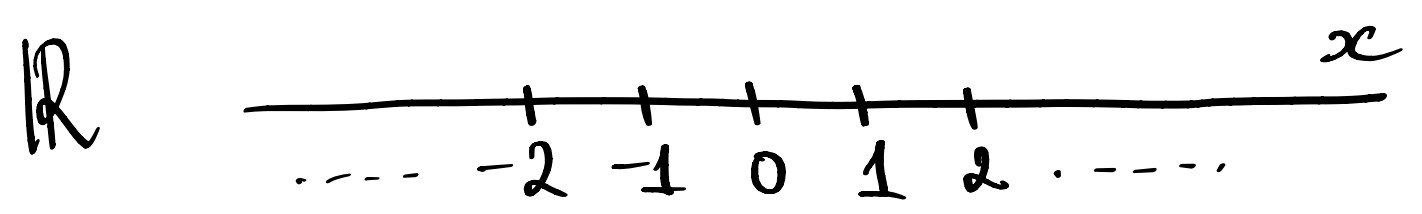
\includegraphics[width=0.5\textwidth]{pictures/one_dimensional_line.jpg}
\end{figure}

Для задания двумерного пространства нужно два числа. Множество всех пар чисел обозначается $\R^2$, читается как ''эр два''. Координаты обозначаются как $(x,y)$. Геометрически это представляется как две прямые, пересекающиеся в своих нулях под прямым углом.

\begin{figure}[h] % [h] означает "здесь"
    \centering
    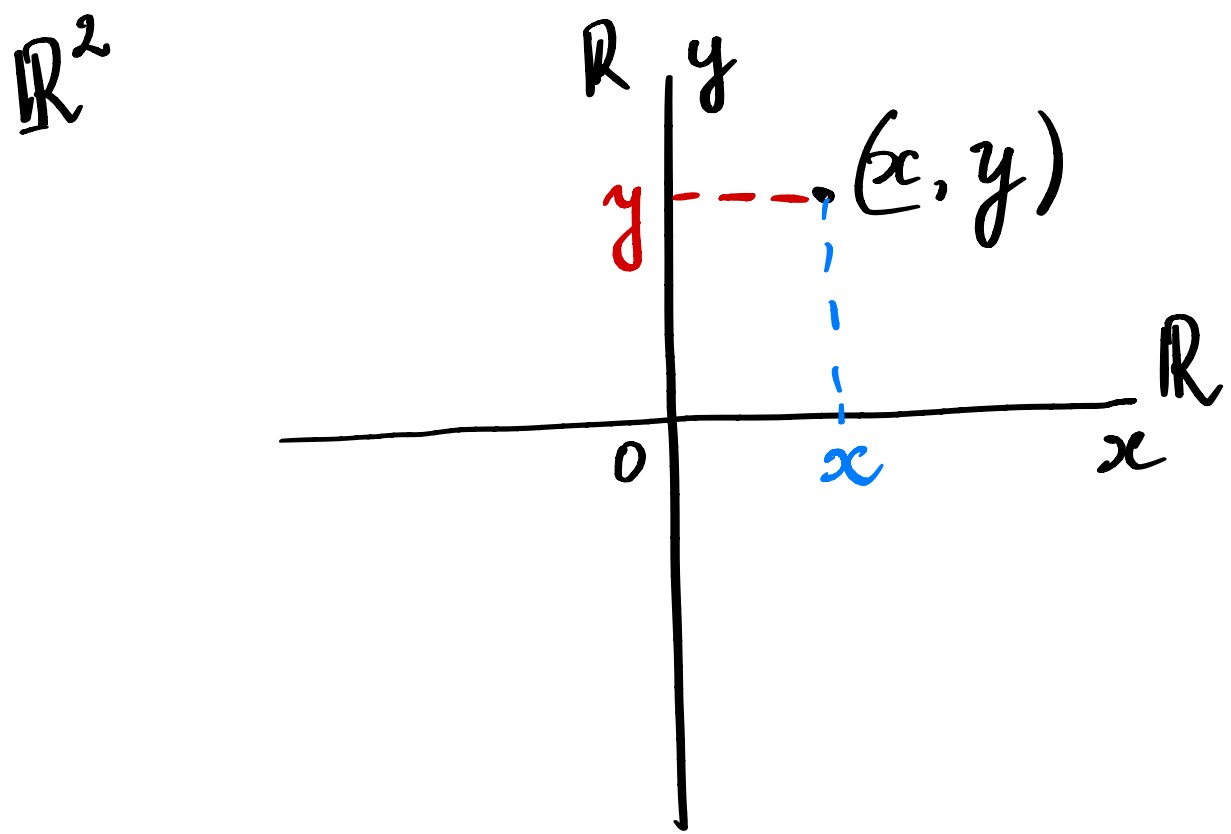
\includegraphics[width=0.5\textwidth]{pictures/two_dimensional_space.jpg}
\end{figure}

Аналогично, для трехмерного пространства $\R^3$ добавляется еще одна прямая, перпендикулярная двум другим. Таким образом, координата точки имеет вид $(x,y,z)$.

\begin{figure}[h] % [h] означает "здесь"
    \centering
    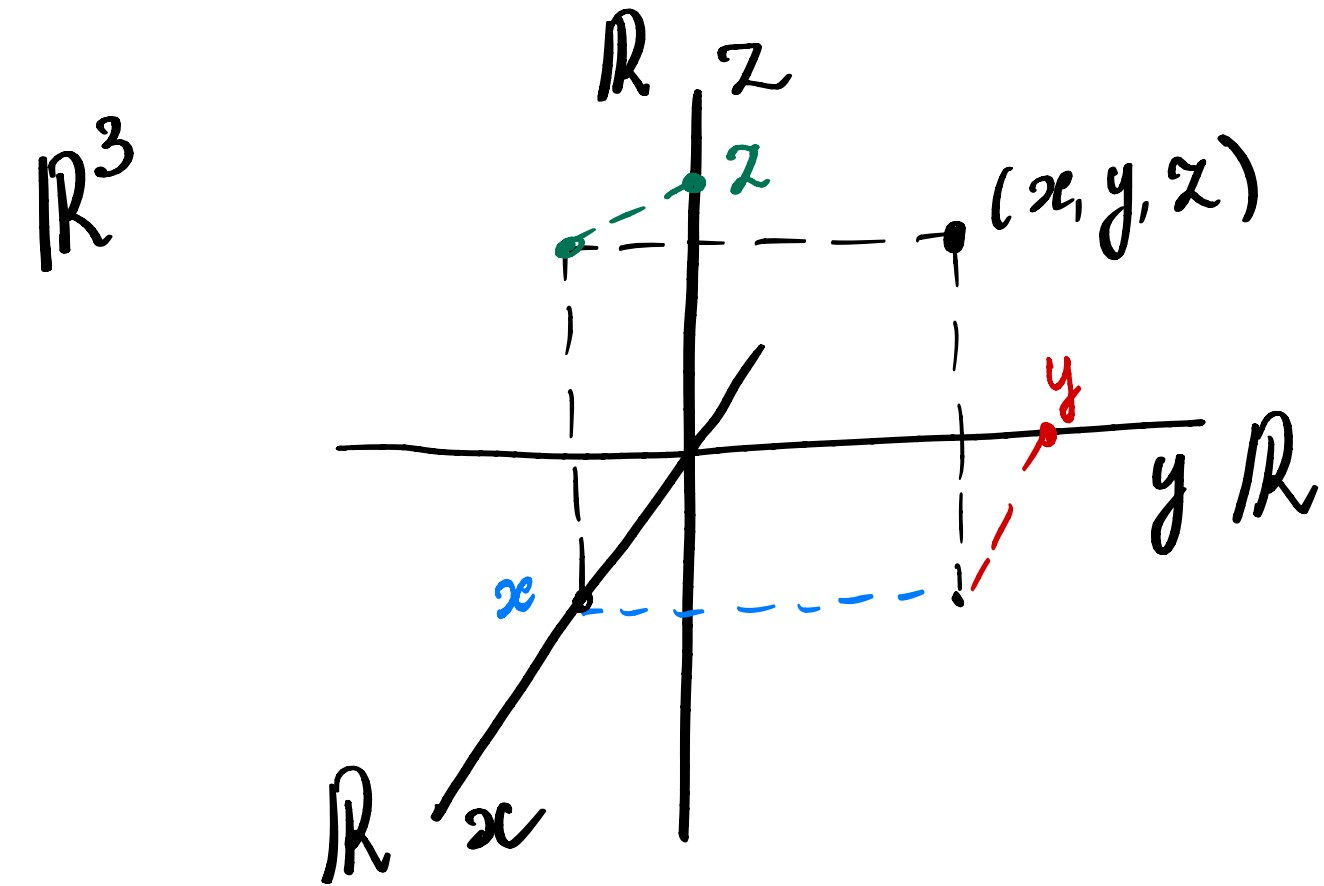
\includegraphics[width=0.5\textwidth]{pictures/three_dimensional_space.jpg}
\end{figure}

\subsection*{FAQ}\addcontentsline{toc}{subsection}{FAQ}

\textbf{С чего это все-таки оси рисуются именно перпендикулярно друг другу?}

Дело в том, что система координат и не обязана быть прямоугольной. Само по себе понятие угла на языке координат будет определено чуть позже, когда мы будем говорить о скалярном произведении векторов. А когда дойдем до матриц, будет ясно, как связаны различные системы координат между собой. Кстати, Декарт в ''Геометрии'' тоже не ограничивался прямоугольными координатами.

Но сейчас мы рассматриваем привычную нам модель описания пространства, где координата точки --- это длина ее проекции на соответствующую координатную прямую (ось).

\noindent\textbf{Зачем пишешь $\R$ на концах?}

Буквы $\R$ рядом с осями я нарисовал, чтобы подчеркнуть, что мы как бы склонировали один и тот же объект (множество чисел) и геометрически их расположили в пространстве. Как правило, так не пишут, и я не буду в дальнейшем, ибо нет смысла.

\noindent\textbf{Какая разница между черными $x,y,z$ и цветными? Это одно и то же?}

Буквы $x, y, z$ на ''концах'' просто указывают, какая переменная бегает по какой из прямых. Цветные $x,y,z$ указывают конкретное значение этих переменных для данной точки. Часто, чтобы не путаться, конкретные значения обозначают с индексом, например, $x_0, y_0, z_0$.

\noindent\textbf{Почему координаты в круглых скобках? В школе/универе/видосах препод писал фигурные/квадратные.}

Координаты самой точки указываются в круглых скобках через запятую. Круглые скобки --- стандартное обозначение упорядоченного набора чисел. На языке программирования можно сказать, что круглые скобки это \textbf{Array}, а фигурные скобки --- \textbf{Set}.

\noindent\textbf{Где стрелочки?}

Стрелки специально не указаны, потому что это задания направления, а про это, думается, лучше поговорить позже, когда обсудим векторы. Хочется, чтобы изложение было последовательным. Таким образом, обращаем внимание на то, что в принципе стрелки тут ни при чем. Важно то, как прямые расположены друг относительно друга.

\noindent\textbf{Важно ли где какая координата? Почему $x,y,z$ именно так нарисованы?}

Да, есть понятие ориентации системы координат. По сути это значит, что направления осей имеют определенное расположение относительно друг друга.

В двумерном случае, традиционно, ось $y$ смотрит вверх, а ось $x$ --- вправо. Если обем осям поменять направление на противоположное, то ориентация не поменяется: ось $y$ смотрит все равно влево относительно оси $x$. А вот если, например, поменять направление только оси $x$, то ориентация, т.е. взаимное расположение осей, изменится.

В трехмерном случае традиционной является такая ориентация, когда ось $y$ смотрит влево относительно $x$ (как и раньше), а ось $z$ смотрит влево относительно $y$. Как бы слепили из двух плоскостей $(x,y)$ и $(y,z)$ одно трехмерное пространство.

Если говорить чуть более формально, то можем дать такое определение. Две системы координат называются одинаково ориентированными, если одну можно непрерывными деформациями перевести в другую. Вернемся к этому вопросу позже, когда дойдем до векторного произведения.

TODO: добавить картинки из Goodnotes.

\noindent\textbf{Есть какой-то всемирный стандарт для этих записей?}

Нет, в математике в принципе нет высеченных в камне стандартов. Например, в C++ можно открыть документацию к версии языка и точно узнать, что и как должно работать. В математике нет создателя/ей (человека по крайней мере), поэтому и документации такой нет. Есть только школы, традиции, которые часто схожи в разных сообществах, но далеко не всегда идентичны.

Так что здесь важно понимать суть. Мы в дальнейшем будем немного по-разному рисовать эти картинки, заодно станет понятно, что тут критично, а что нет.

\section*{Функции}\addcontentsline{toc}{section}{Функции}
\subsection*{Функция как формула}\addcontentsline{toc}{subsection}{Функция как формула}
История развития понятия функции в общем-то очень переплетается с сюжетом про Декарта, Ньютона и Эйлера из раздела про системы координат.

Как уже говорилось, Декарт и Ферма начали описывать геометрические кривые алгебраическими уравнениями. Так как кривые рассматривались на плоскости, то уравнения имели две переменные $x,y$. Но что означает уравнение двух переменных?

Посмотрим на примере уравнения прямой:
\[
ax+by + c= 0
\]
Решения этого уравнения это все пары:
\[
(x, -\frac{ax +c}{b})
\]
Чтобы найти это решение мы \textit{выразили} $y$ через $x$:
\[
y = -\frac{ax+c}{b}
\]

Эйлер в ''Анализе бесконечных'' называл $y$ функцией $x$, если $y$ задан формулой, в которую входят только переменная $x$ и константы, например,
\[
y = 4x^5 - \sqrt{x} + \frac{x}{\sqrt{x+3}}.
\]

Поэтому, по сути, в этом формульном смысле понятие функции витает и у Декарта, так как он прекрасно понимал, что уравнение задает зависимость между переменными. Но самого слова ''функция'' тогда еще не было. Ньютон, опять же, уже фактически использовал функциональную нотацию, указывая зависимость между величинами. Но как математический объект, определение функции дал Эйлер.

\begin{figure}[h] % [h] означает "здесь"
    \centering
    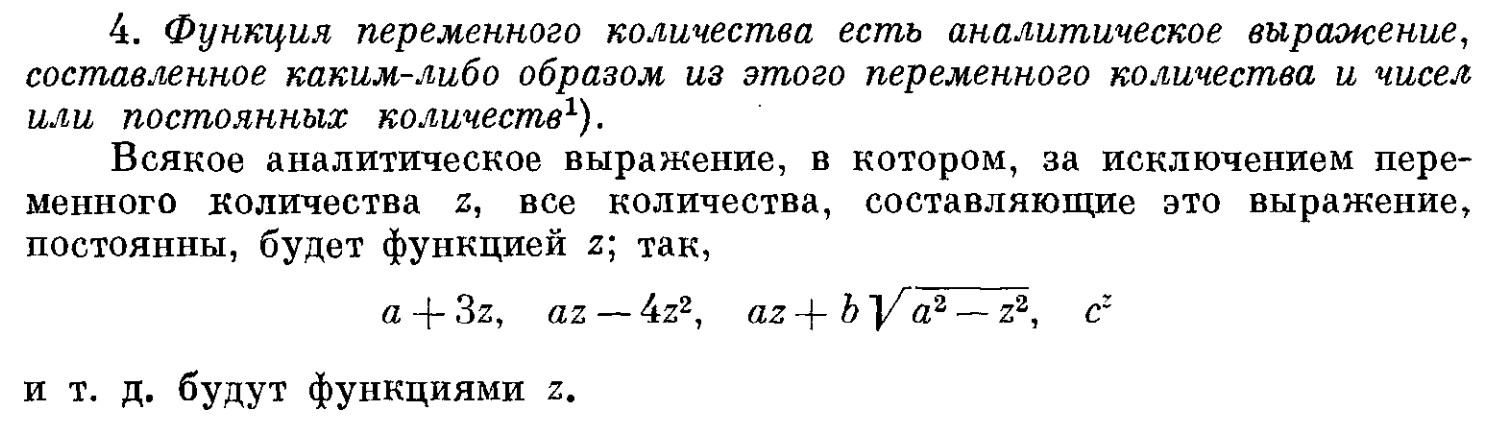
\includegraphics[width=0.8\textwidth]{pictures/eulers_function_def.jpg}
    \caption{Определение функции из ''Анализа бесконечных'' Эйлера (1748) \cite{EulerInfiniteV1}}
\end{figure}

\subsection*{Функция как соответствие}\addcontentsline{toc}{subsection}{Функция как соответствие}

Такое определение для обычного школьника было бы вполне привычным, но в дальнейшем представление о функции становилось более широким, чем просто формула.

Ключевая суть функции заключается в том, что она устанавливает взаимосвязь между переменными. Например, можно определить зависимость положения Солнца относительно времени на часах. Или величину зарплаты в зависимости от грейда. На уровне идеи формулы никакой нет. И хотя часто зависимость можно выразить формулой, есть риск, что все же от такого подхода мы что-то теряем.

И действительно, как сейчас известно, не любую функцию можно выразить формулой (как говорят, выразить ''в радикалах''), да и не всегда это нужно.

Поэтому, где-то с работ Гаусса и Дирихле (18 век), начало формироваться представление о функции как о правиле, по которому одному или нескольким параметрам сопоставляется некий результат.

\begin{figure}[h] % [h] означает "здесь"
    \centering
    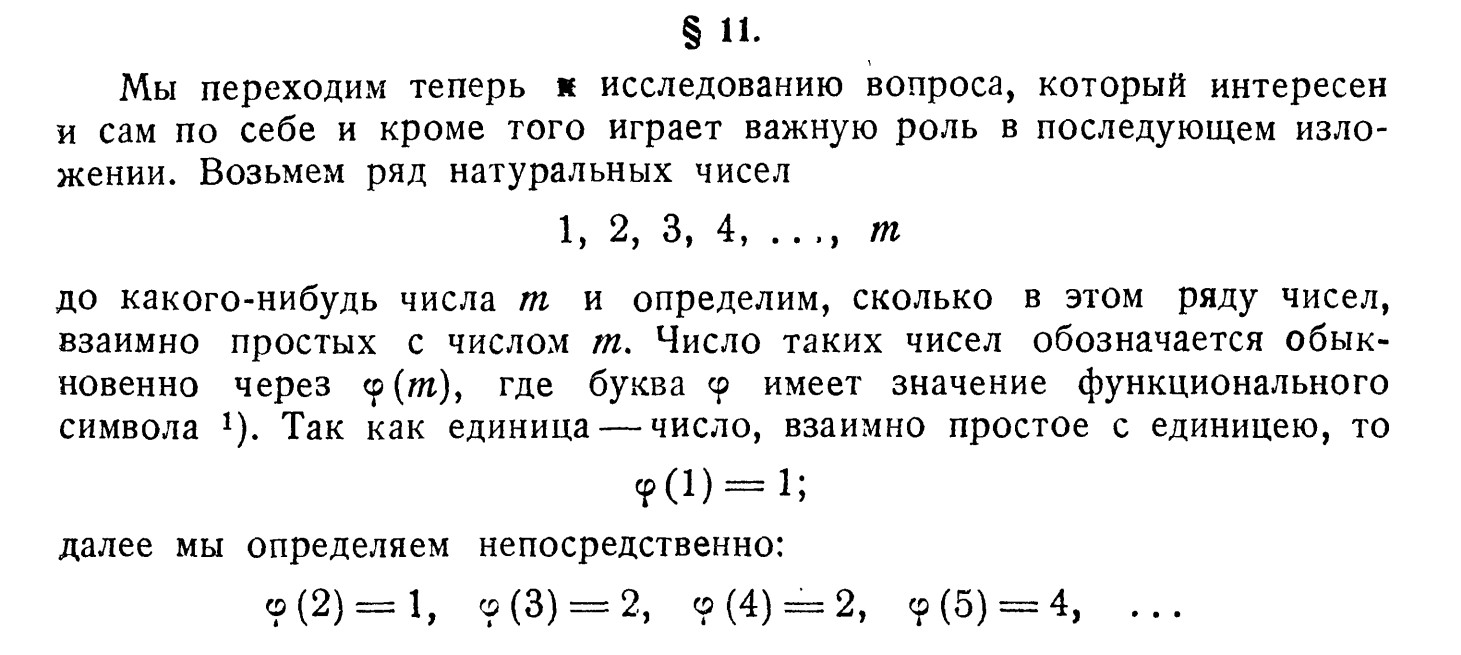
\includegraphics[width=0.8\textwidth]{pictures/euler_function_by_dirichlet.jpg}
    \caption{Определение \href{https://w.wiki/EsaF}{функции Эйлера} в лекциях Дирихле \cite{DirichletNumberTheoryLectures}}
\end{figure}

Как уже говорилось во введении, нетворк --- это пример функции, которая по нетворк--параметрам преобразовывает трансформации анимационных объектов. И формулу для него на листочке записывать --- идея страшная.

TODO: рисунок схематично иллюстрирующий нетворк.

\threestars

Традиционно, функцию обозначают буквой $f$, а ее аргумент --- буквой $x$. Значение функции $f$ при заданном $x \in \R$ обозначается символом $f(x)$. Чтобы сразу указать, какие обозначения для конкретной функции будут использоваться, часто говорят ''задана функция $f(x)$''.

Есть мнение, что таких фраз нужно избегать, потому что это неграмотно: если написал $f(x)$, то это уже не функция, а значение функции в точке $x$. Тогда пишут либо просто $f$, либо $f(\cdot)$, если хотят подчеркнуть, что аргумент один.

Когда говорят о функции, важно понимать, какая у нее область определения, т.е. какие именно аргументы можно подставлять в функцию, чтобы получать корректное значение. Поэтому говорят ''функция $f$, определенная на отрезке $[0,1]$'' и т.п.

В программировании есть assert-ы. Это проверки, обычно в начале функции, что некоторое условие на входящие параметры выполнено. Если условие не выполнено, кидается ошибка. По сути, это и есть задание области определения функции.

TODO: добавить примеры?.

\subsection*{График функции}\addcontentsline{toc}{subsection}{График функции}
Функция --- это понятие, делающее еще один шаг в сторону от геометрии к алгебре (привет Декарту) и далее к анализу (привет Эйлеру). Но интуиция и наглядность, присущая геометрии --- никуда не денешься --- вещь важная. Формула --- хорошо, а формула с рисунком --- еще лучше! Особенно, если ты физик, как Ньютон.

TODO: вставить картинку из Начал.

График функции является, наверное, главным виновником популярности именно прямоугольных осей координат. Для чего нужен график? Чтобы иллюстрировать то, как изменяется одна величина при изменении другой/других. И если функция числовая, т.е. принимает числовые значения (что вообще-то не обязательно), то логично изображать ее значения как бы столбиками, стоящими на аргументах функции. Все столбики, ясное дело, параллельны и стоят они все на одном уровне. Вот и получается сама собой прямоугольная система координат и привычный рисунок.

\df Графиком функции $f$, определенной на множестве $X$, называется множество пар $\{(x,f(x))\}_{x \in X}$. Простыми словами, взяли все значения переменной $x \in X$, посчитали от них значения $f(x)$ и записали все результаты в табличку:
\begin{center}
\begin{tabular}{|c|c|c|c|c|c|}
\hline
$x$ & $x_1$ & $x_2$ & $x_3$ & $x_4$ & $\cdots$ \\
\hline
$f(x)$  & $y_1$ & $y_2$ & $y_3$ & $y_4$ & $\cdots$\\
\hline
\end{tabular}
\end{center}
Для наглядного изображения графика функции удобнее всего нарисовать картинку, где все эти точки образуют гладкую кривую линию:

\begin{figure}[h] % [h] означает "здесь"
    \centering
    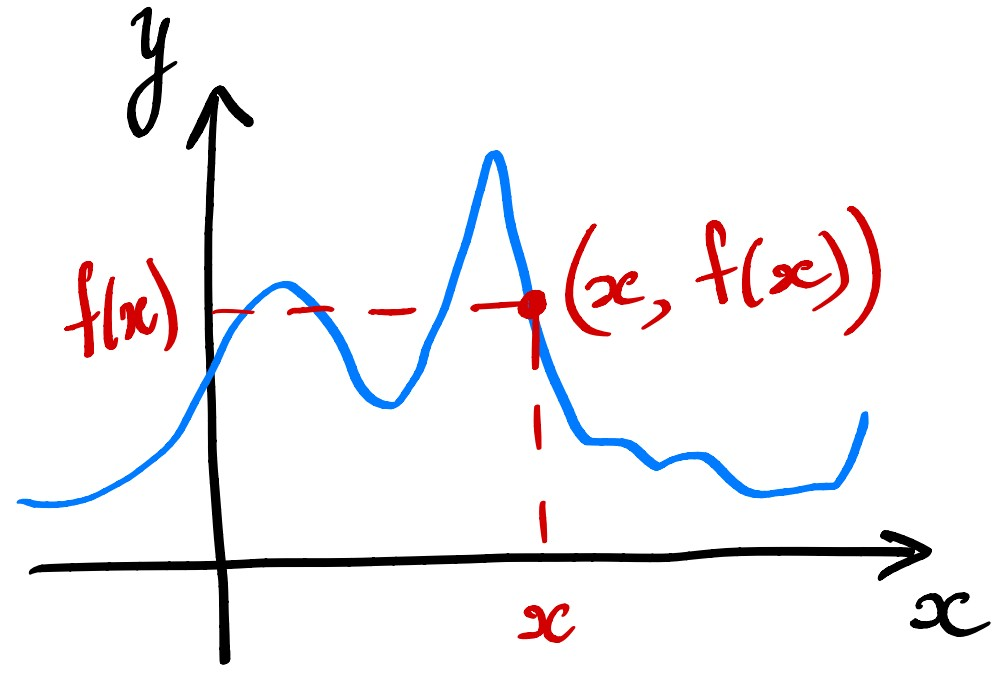
\includegraphics[width=0.5\textwidth]{pictures/pct_function_plot.jpg}
\end{figure}

Так что, строго говоря, как и система координат, график не является ''рисунком'', это не геометрический объект, а множество пар аргумент+значение. Но это множество традиционно иллюстрируют в виде рисунка в прямоугольной системе координат.

\NB{Конечно, график далеко не обязан быть гладким и даже непрерывным. Отсюда возникают строгие понятия, характеризующие функцию, которые образуют теорию под названием анализ функций (по-народному ''матан'').}

\subsection*{Кривые и поверхности как графики функций}\addcontentsline{toc}{subsection}{Кривые и поверхности как графики функций}

Может возникнуть мысль, что график функции нужен просто ради наглядной картинки. Это отчасти так, но здесь опять проявляется связь алгебраического и геометрического. С одной стороны, по функции, негеометрическому объекту, можно построить график, который не только дает интуитивное графическое представление о ней, но и является уже описанием геометрического объекта: кривой, поверхности и т.п.

\threestars

Например, мы знаем, что окружность радиуса 1 задается уравнением
\[
x^2 + y^2 = 1.
\]
Выразим $y$ через $x$:
\[
y^2 = 1 - x^2,
\]
значит,
\[
y = \sqrt{1-x^2} \qquad \text{или}\qquad y = -\sqrt{1-x^2}.
\]

Здесь мы получили две функции $f_1(x) = \sqrt{1-x^2}$ и $f_2(x) = -\sqrt{1-x^2}$. Построим их графики:

\begin{figure}[h] % [h] означает "здесь"
    \centering
    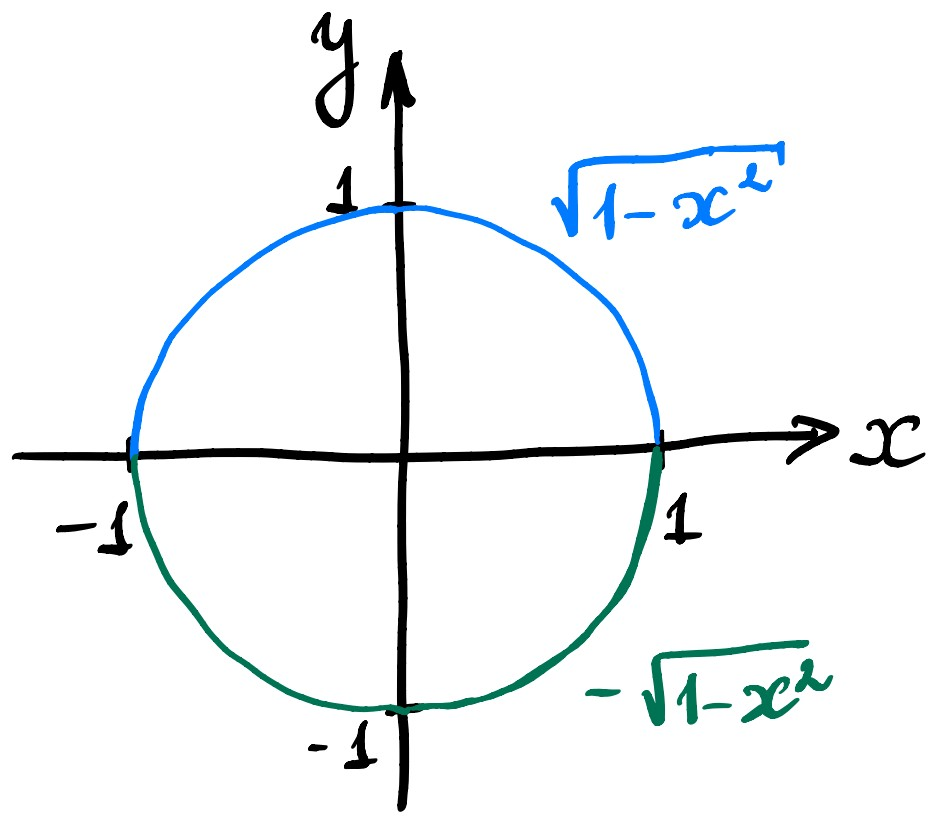
\includegraphics[width=0.5\textwidth]{pictures/pct_circle_plot.jpg}
\end{figure}

Мы видим, что два этих графика в объединении дают геометрический объект --- окружность. И так можно делать с любыми кривыми на плоскости, если они не слишком экзотические.

\threestars

Аналогично, можно рассмотреть уравнение единичной сферы
\[
x^2 + y^2 + z^2 = 1.
\]
Выразим $z^2$:
\[
z^2 = 1 - x^2 - y^2
\]
откуда
\[
z = \sqrt{1-x^2 - y^2} \qquad \text{или}\qquad z = -\sqrt{1-x^2 - y^2}.
\]

Графиками функций $f_1(x,y) = \sqrt{1-x^2 - y^2}$ и $f_2(x,y) = -\sqrt{1-x^2 - y^2}$ будут две полусферы.

\begin{figure}[H]
    \centering
    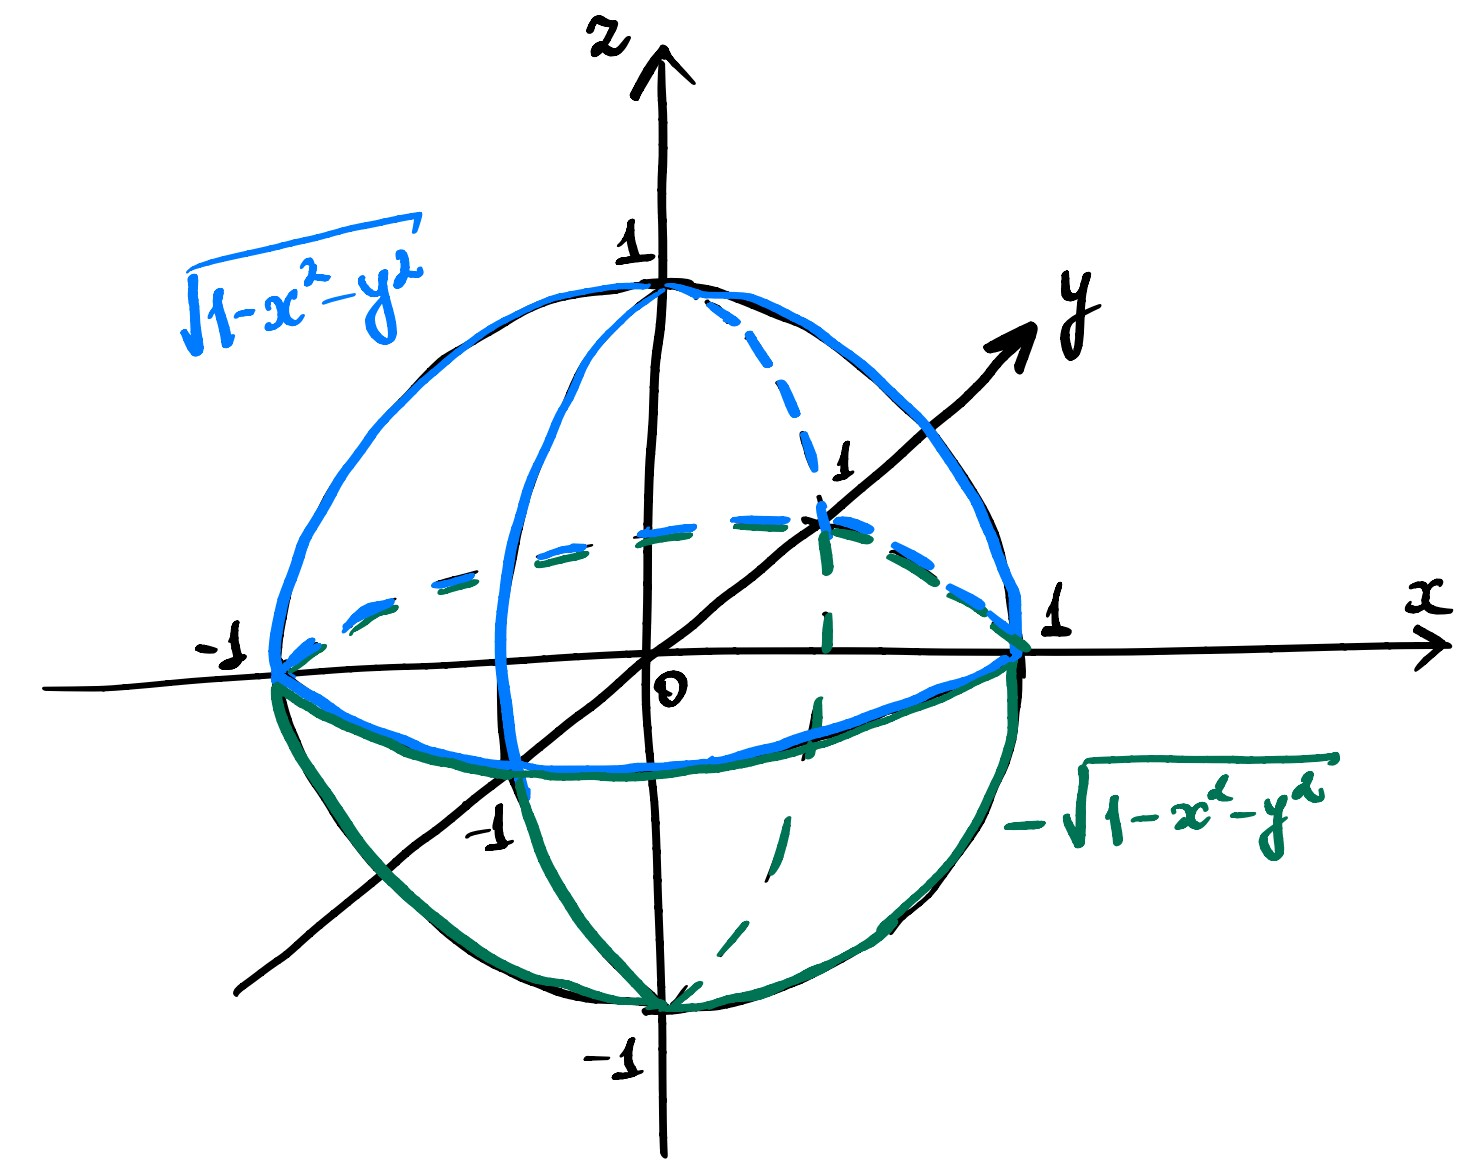
\includegraphics[width=0.5\textwidth]{pictures/pct_sphere_plot.jpg}
\end{figure}

\subsection*{Примеры функций и их графиков}\addcontentsline{toc}{subsection}{Примеры функций и их графиков}

\subpoint{Константа}
Функция, которая всюду принимает одно значение, называется константой.
\[
f(x) = C, \quad \text{где } C \in \R - \text{число}.
\]
\begin{figure}[H]
    \centering
    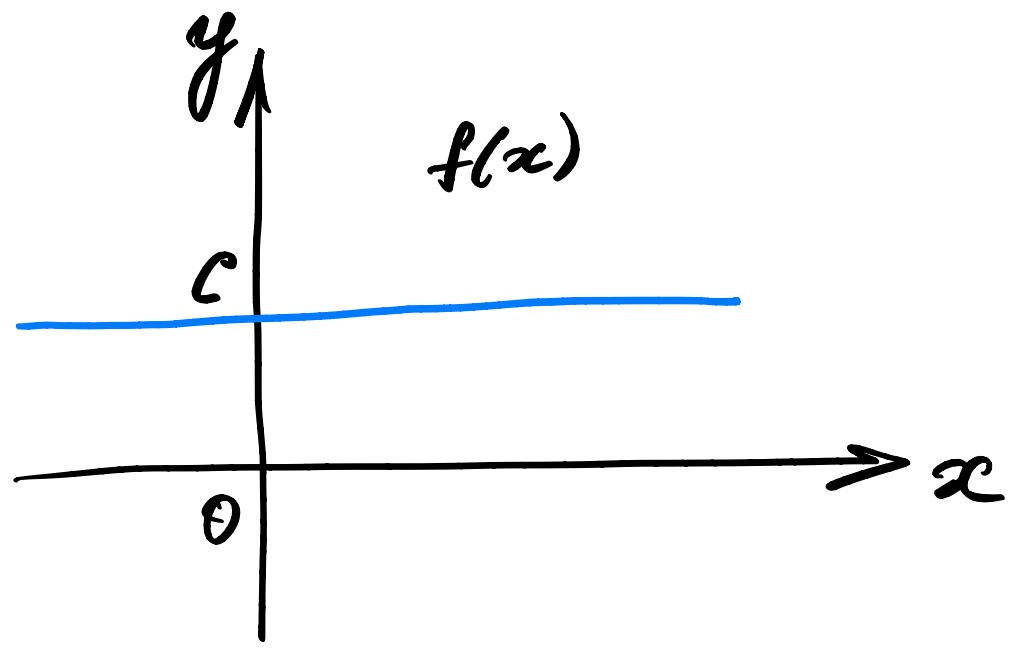
\includegraphics[width=0.4\textwidth]{pictures/pct_const_plot.jpg}
\end{figure}
\subpoint{Тождественная функция}
Функция, которая возвращает то же значение, которое получила на вход, называется тождественной.
\[f(x) = x\]
\begin{figure}[H]
    \centering
    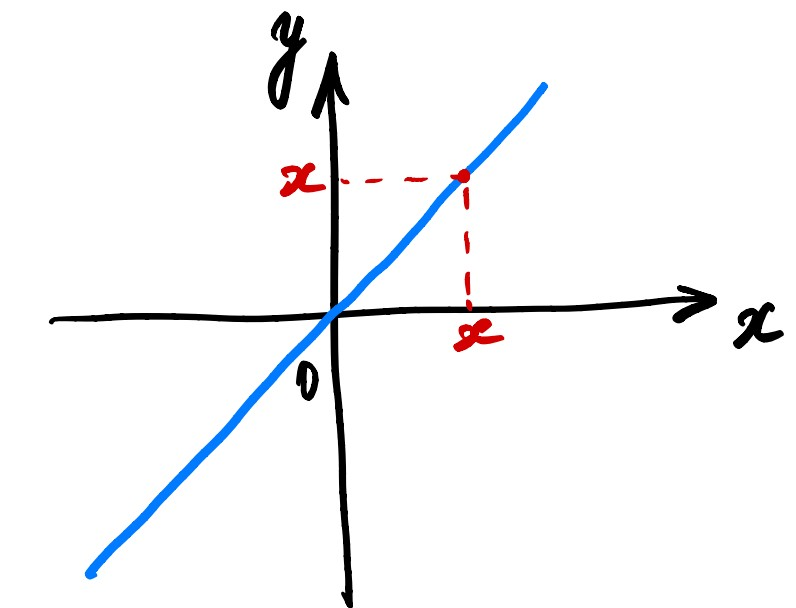
\includegraphics[width=0.35\textwidth]{pictures/pct_identity_function_plot.jpg}
\end{figure}
\subpoint{Степенная функция}
Степенная функция определяется формулой
\[
f(x) = x^a, \quad a\in\R.
\]
\begin{figure}[H]
    \centering
    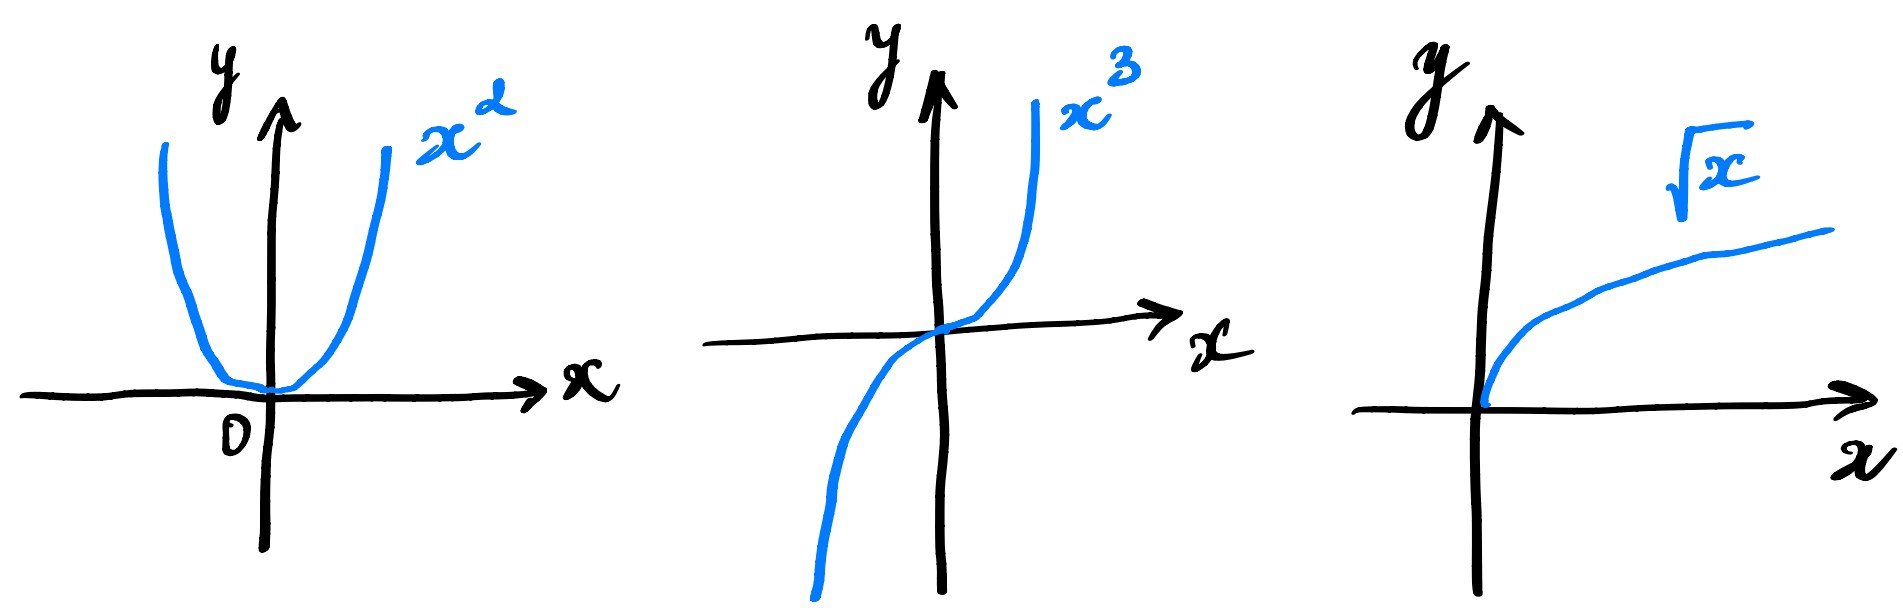
\includegraphics[width=0.7\textwidth]{pictures/pct_degree_function_plot.jpg}
\end{figure}

При разных значениях параметра $a$ будут получаться различные функции:
\begin{align*}
    &a=0 \Rightarrow f(x) = 1\\
    &a=1 \Rightarrow f(x) = x\\
    &a=2 \Rightarrow f(x) = x^2\\
    &a=\frac{1}{2} \Rightarrow f(x) = \sqrt{x}
\end{align*}
\subpoint{Показательная функция}
Показательная функция определяется формулой
\[
f(x) = a^x, \quad a \ge 0.
\]
\begin{figure}[H]
    \centering
    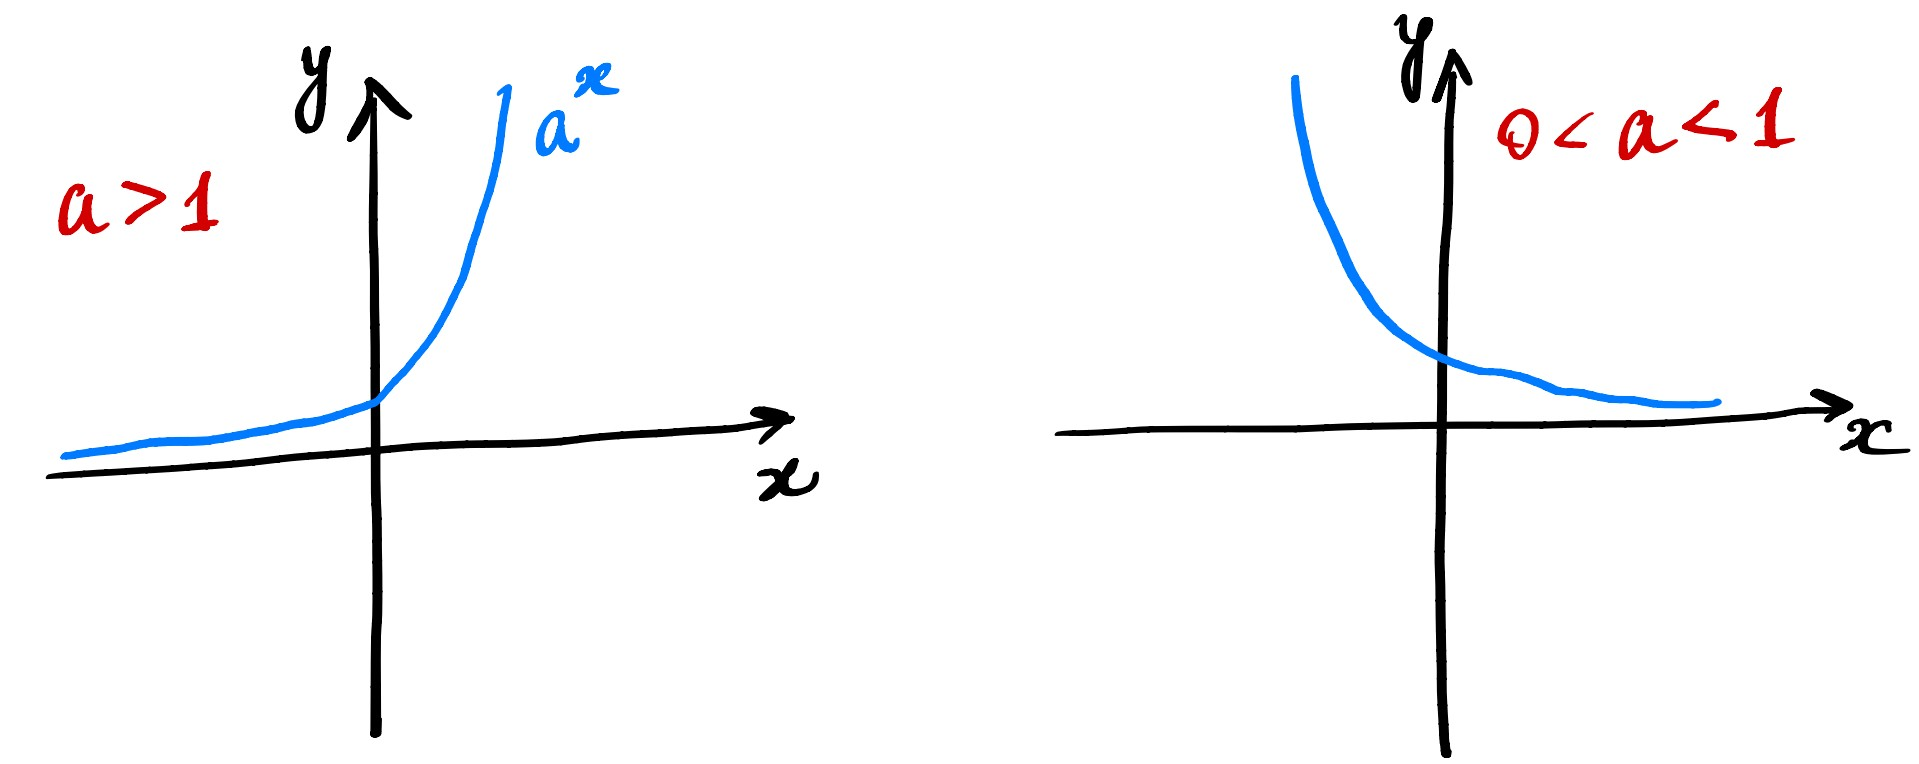
\includegraphics[width=0.6\textwidth]{pictures/pct_exp_function_plot.jpg}
\end{figure}

\NB{Частный случай $a=e$ дает функцию
\[
f(x) = e^x,
\]
которая называется экспонентой.}
\subpoint{Тригонометрические функции}
О тригонометрических функциях подробнее мы поговорим ниже, а пока просто посмотрим на их графики
\begin{figure}[H]
    \centering
    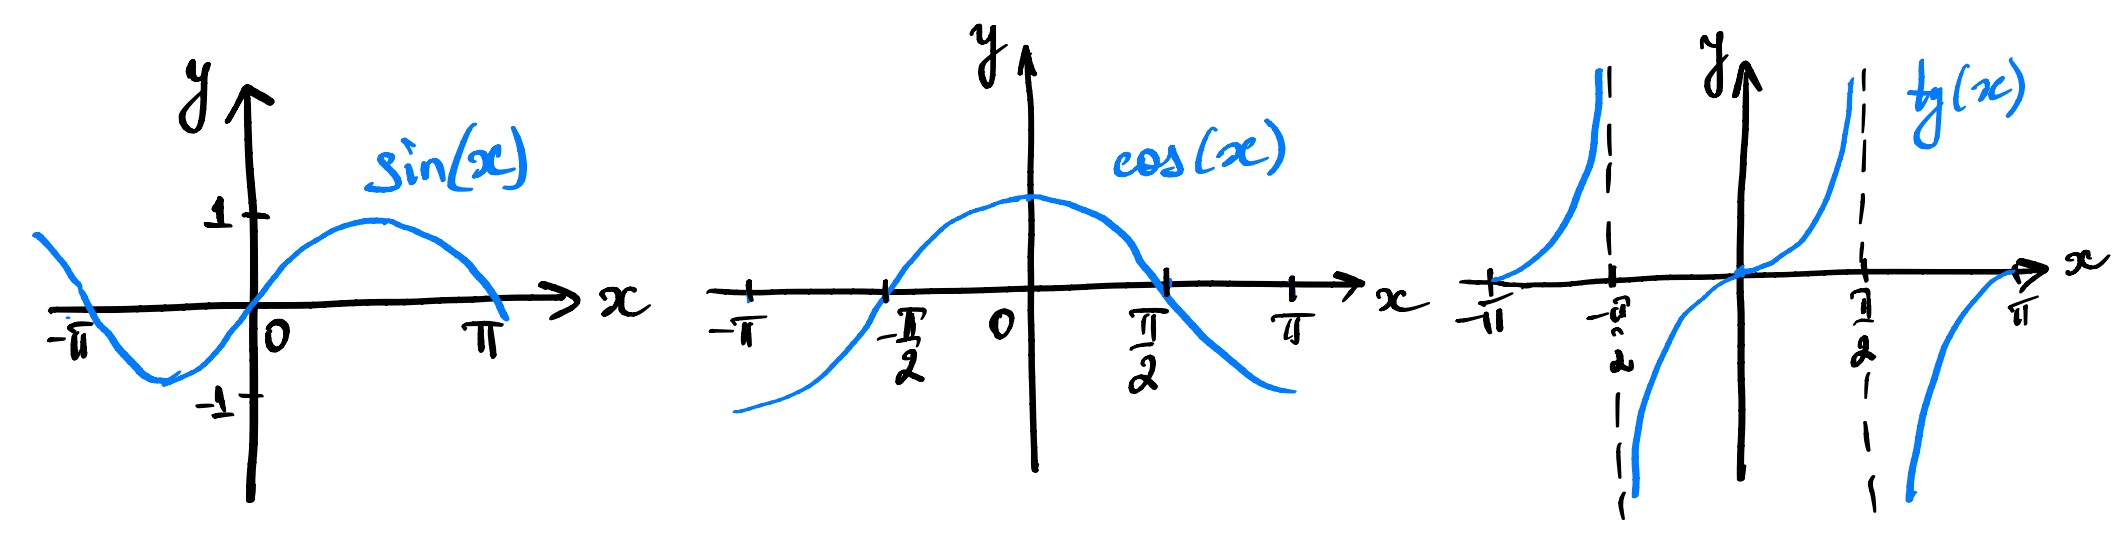
\includegraphics[width=0.9\textwidth]{pictures/pct_trigonometry_functions_plots.jpg}
\end{figure}

\section*{Тригонометрия}\addcontentsline{toc}{section}{Тригонометрия}
\subsection*{Мотивация}\addcontentsline{toc}{subsection}{Мотивация}
% Для того, чтобы понять, зачем нужна тригонометрия и все эти мутные всем известные функции, нужно задаться одним вопросом --- что такое угол? И вообще зачем это понятие вводить? Ведь 

% Угол не может быть без двух лучей или отрезков, отложенных от одной точки. 

% TODO: покопать историю и привести примеры физических задач, где возникает тригонометрия (мб закон движения маятника, волны).

Как говорилось выше, геометрия изучает метрические свойства фигур в плоскости или пространстве. Под фигурами можно понимать то, что можно изобразить, нарисовать. Например, прямые, кривые, окружности, эллипсы, сферы, параллелепипеды, сечения одних фигур другими и т.д.

Естественным историческим ходом развития мысли в геометрии выделялись более узкие направления. Так, известно, что в Египте строились пирамиды (3000 лет до н.э.), где требовались рассчеты длин и углов в треугольнике для того чтобы понять сколько материалов нужно для выстраивания пирамиды определенных размеров.

Затем греческие астрономы (190-120 лет до н.э.) стали замечать, что Солнце каждый день встает немного смещаясь в восток, и скоро поняли, что Солнце движется относительно Земли по окружности, а полный круг делает за год. Отсюда пошло разделение полного оборота вокруг своей оси на 360 градусов. Встал вопрос, а какого радиуса эта окружность, т.е. на каком расстоянии Солнце находится от Земли. Выяснилось, что эта задача решается через построения прямоугольных треугольников и поиска в них длин сторон и углов.

Таким образом, стала выкристализовываться тригонометрия -- геометрия треугольников. Впрочем, такой взгляд скорее вреден, поскольку сейчас известно о приложениях тригонометрии в совершенно далеких друг от друга областях, от астрономии, механики, электричества до методов сжатия изображений.

Об истории тригонометрии и о ее красивых приложениях есть 40-минутная лекция канадского историка математики Glen Van Brummelen \href{https://youtu.be/eurWRYY82AQ?si=FBo6oCkqklM5nc1_}{The Story of Trigonometry: Revolutions in the Heavens, and on the Earth}. Для демонстрации он там использует сайт \href{https://www.myphysicslab.com/}{MyPhysicsLab}.

\subsection*{Отношения в прямоугольном треугольнике}\addcontentsline{toc}{subsection}{Отношения в прямоугольном треугольнике}
Изобразим прямоугольный треугольник $\triangle ABC$ с прямым углом $\angle C$ и сторонами $a,b,c$. Обозначим угол $\angle A = \alpha$.
\begin{figure}[H]
    \centering
    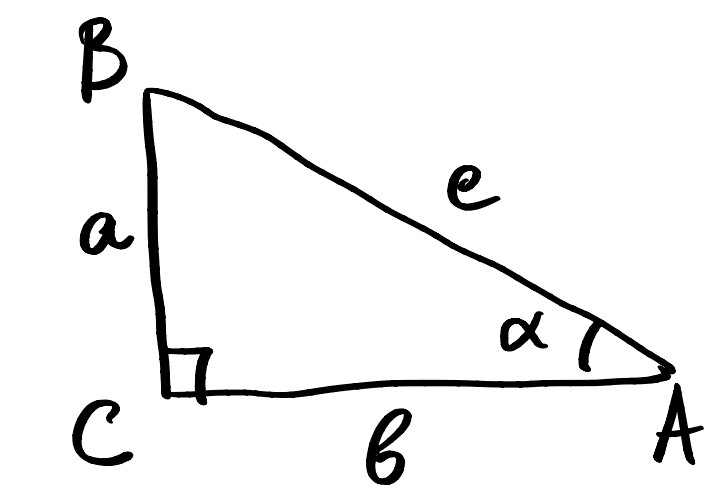
\includegraphics[width=0.25\textwidth]{pictures/pct_triangle_trigonometry.jpg}
\end{figure}

Тогда по определению синус (sine), косинус (cosine), тангенс (tangent) и котангенс (cotangent) угла $\alpha$ есть отношения сторон:
\begin{align*}
    &\sin \alpha = \frac{a}{c}\\
    &\cos \alpha = \frac{b}{c}\\
    &\tg \alpha = \frac{a}{b}\\
    &\ctg \alpha = \frac{b}{a} = \frac{1}{\tg \alpha}
\end{align*}

Отметим свойства, следующие из этого определения
\begin{itemize}
    \item $0 \le \sin \alpha \le 1$, \ \  $0\le \cos \alpha \le 1$
    \item $\sin^2\alpha + \cos^2 \alpha = \frac{a^2}{c^2} + \frac{b^2}{c^2} = \frac{a^2 +b^2}{c^2} \frac{c^2}{c^2}= 1$ (теорема Пифагора)
    \item $b = c \cdot \cos\alpha$ -- проекция $AB$ на прямую $AC$
\end{itemize}

\subsection*{Точка на окружности}\addcontentsline{toc}{subsection}{Точка на окружности}
Теперь совершим эволюционный переход от египтян и вавилонян к грекам, и определим тригонометрические функции, связав их с геометрией окружности единичного радиуса.

Итак, рассмотрим окружность радиуса 1 и поместим ее в начало прямоугольной системы координат. Затем возьмем произвольную точку $P$ на этой окружности, соединим ее с центром окружности и обозначим получившийся угол за $\alpha$.

Тогда по определению синусом угла $\alpha$ называется координата $y$ точки $P$, а косинусом -- координата $x$.

\begin{figure}[H]
    \centering
    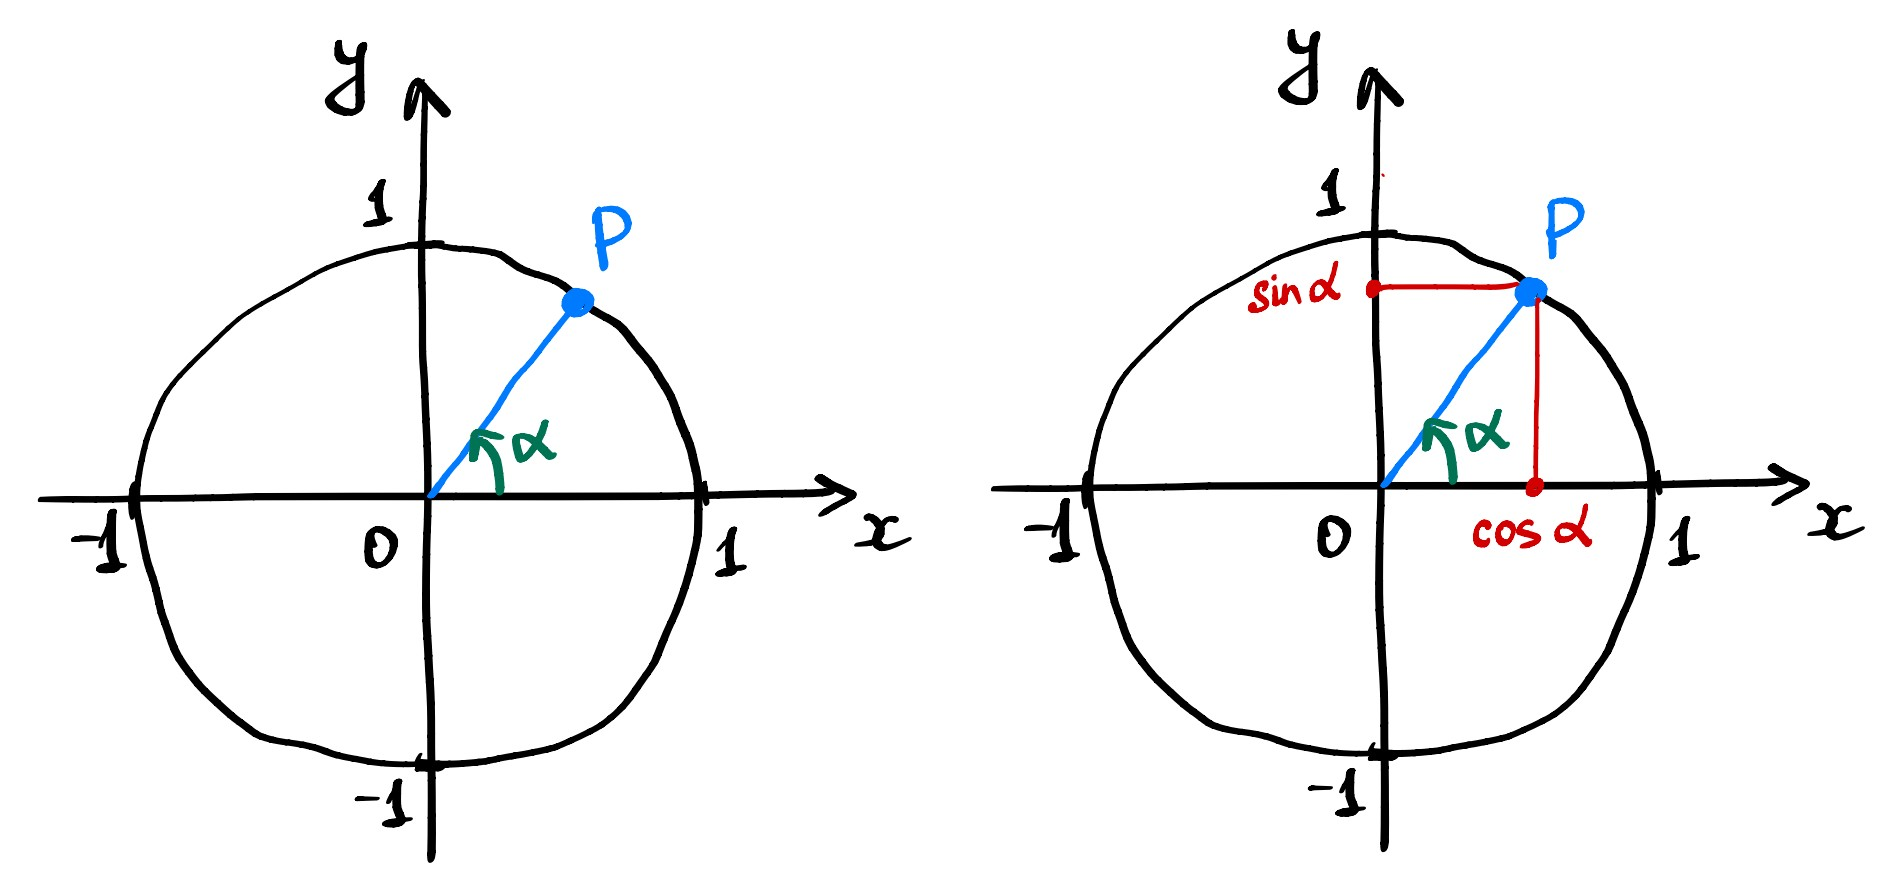
\includegraphics[width=0.9\textwidth]{pictures/pct_sin_cos_1.jpg}
\end{figure}

Но это еще не все. Проведем касательную к точке $P$ и продлим ее до пересечения с осями системы координат. Тогда тангенсом называется длина отрезка от точки $P$ до пересечения с осью абсцисс, а котангенсом называется длина отрезка от точки $P$ до пересечения с осью ординат.

\begin{figure}[H]
    \centering
    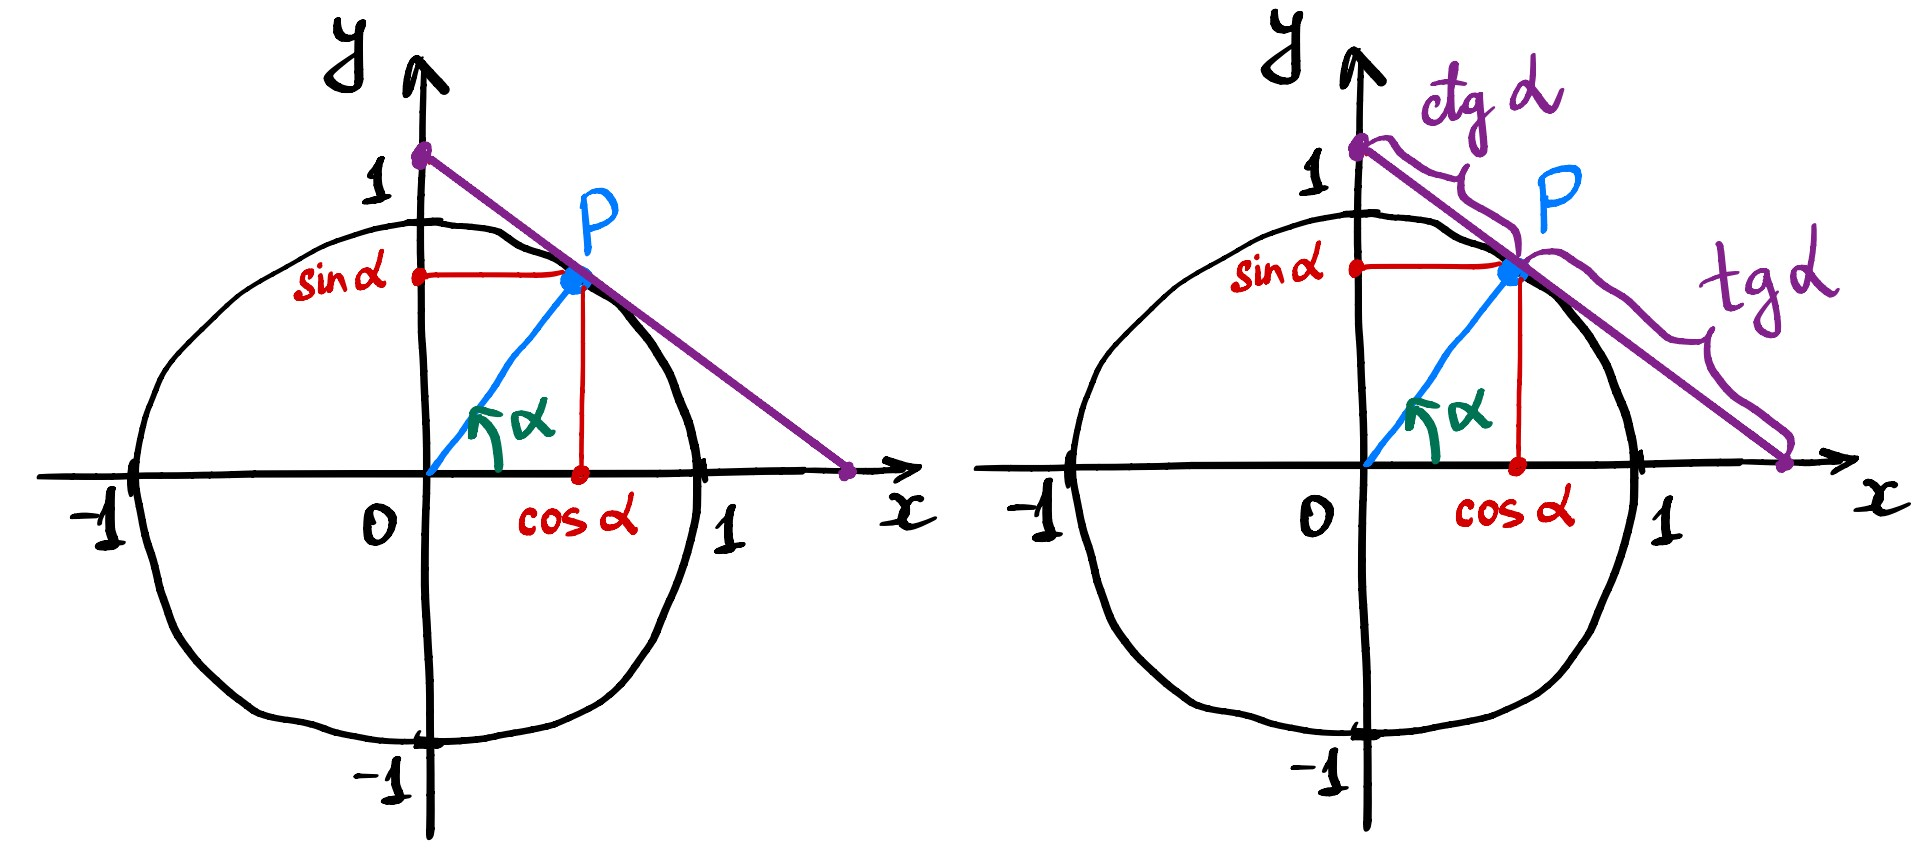
\includegraphics[width=0.9\textwidth]{pictures/pct_sin_cos_2.jpg}
\end{figure}

Вот так с одной стороны определение получается более сложным: используется окружность, координаты, проводится касательная. А с другой стороны, такой взгляд будто открывает глубину понятий. Слово синус в греческом языке означает ''хорда''. И действительно, мы видим по рисунку, что синус это половина длины хорды, а косинус (ко-синус!) половина длины смежной хорды.

Тангенс означает ''касание''. И мы видим, что тангенс это просто длина части касательной. А котангенс (ко-тангенс!) -- другая часть этой же касательной.

Рекомендую посмотреть об этом видео \href{https://youtu.be/snHKEpCv0Hk?si=6_w2j3Dbjdi4dpH5}{Beautiful Trigonometry} от Numberphile.

\threestars

Теперь отметим, что при определении тригонометрических функций через окружность, они могут принимать и отрицательные значения. Так,
\begin{align*}
    &-1 \le \sin \alpha \le 1\\
    &-1 \le \cos \alpha \le 1
\end{align*}
Сразу же видны и многие другие важные свойства, которые в школе часто пытаются зубрить:
\begin{itemize}
    \item периодичность: $\sin(\alpha) = \sin(\alpha + 2\pi)$
    \item нечетность синуса: $\sin(-\alpha) = - \sin \alpha$
    \item четность косинуса: $\cos(-\alpha) = \cos \alpha$
    \item $\sin(\alpha + \pi) = -\sin \alpha$
    \item $\sin(\alpha + \frac{\pi}{2}) = -\cos \alpha$
\end{itemize}
и так далее. Учить тяжело и не нужно, но понимать легко и полезно.

\subsection*{Графики}\addcontentsline{toc}{subsection}{Графики}
Итак, определения синуса, косинуса, тангенса и котангенса через единичную окружность задают числовые функции
\[\sin(x), \quad \cos(x),\quad \tg(x), \quad \ctg(x),\]
причем если $\sin(x)$ и $\cos(x)$ определены на всей числовой прямой, то $\tg(x)$ и $\ctg(x)$ имеют неопределенности.

Нарисуем график синуса.
\begin{figure}[H]
    \centering
    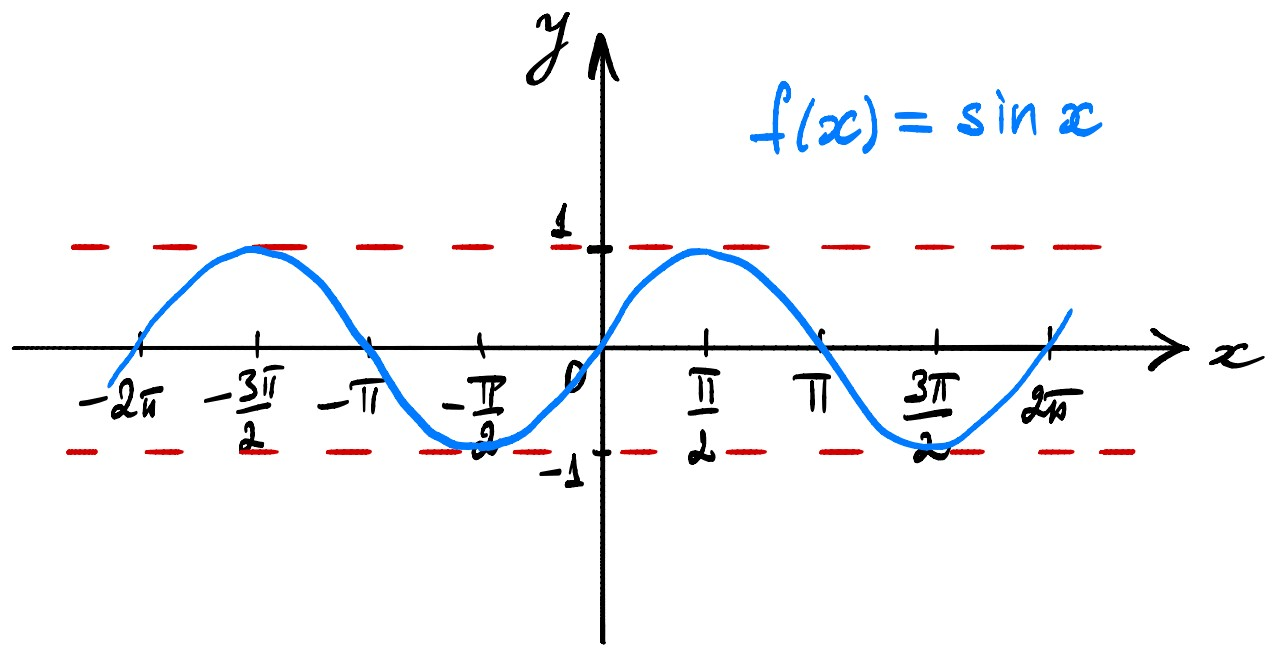
\includegraphics[width=0.6\textwidth]{pictures/pct_sinus_plot.jpg}
\end{figure}

Полученная кривая напоминает волну. Она постоянно колеблется между максимальным и минимальным значениями, причем, подходя к ним, плавно замедляется, а отдаляясь, также плавно ускоряется.

График косинуса ничем не отличается от синуса, кроме сдвига на $\pi/2$ по горизонтали. Это видно из построения косинуса на окружности.

\begin{figure}[H]
    \centering
    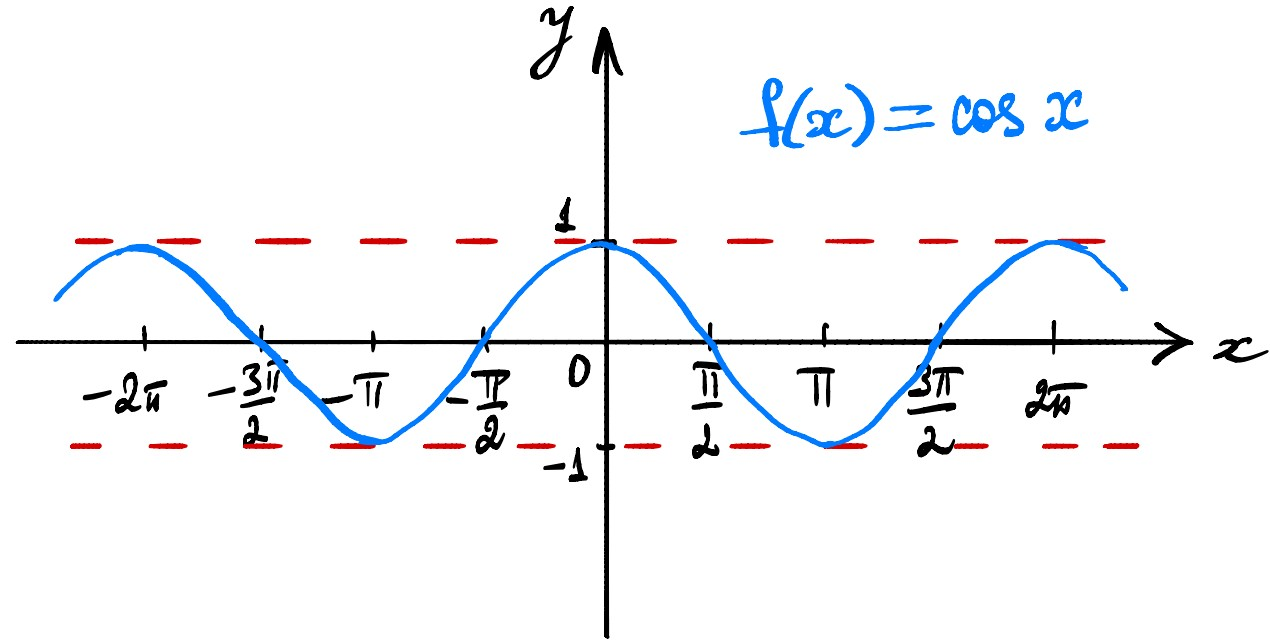
\includegraphics[width=0.6\textwidth]{pictures/pct_cosinus_plot.jpg}
\end{figure}

\threestars

Тангенс и котангенс имеют также схожие между собой графики, однако отличные от графиков синуса и косинуса.
\begin{figure}[H]
    \centering
    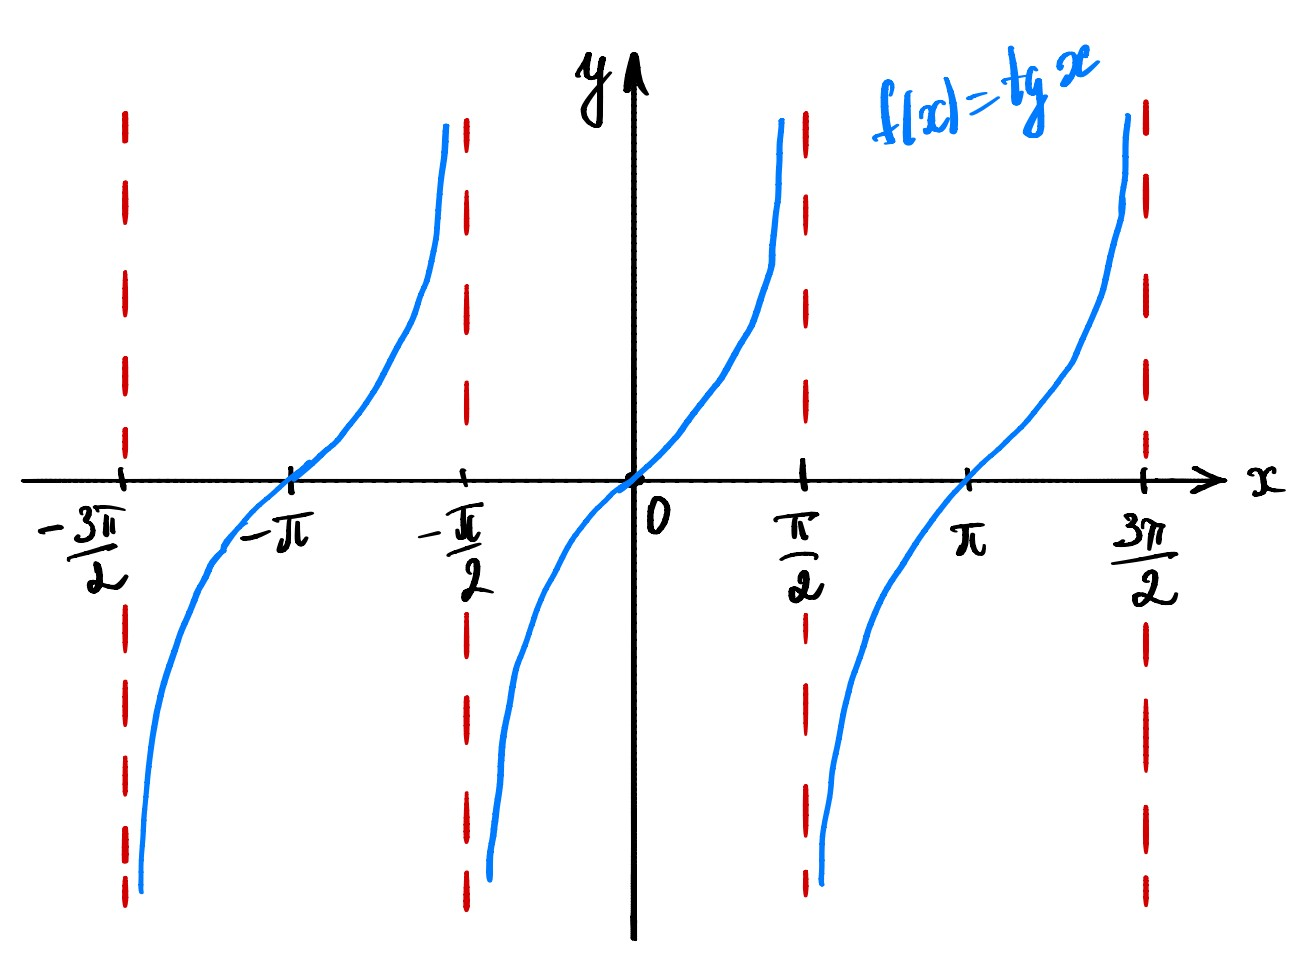
\includegraphics[width=0.6\textwidth]{pictures/pct_tangence_plot.jpg}
\end{figure}

\begin{figure}[H]
    \centering
    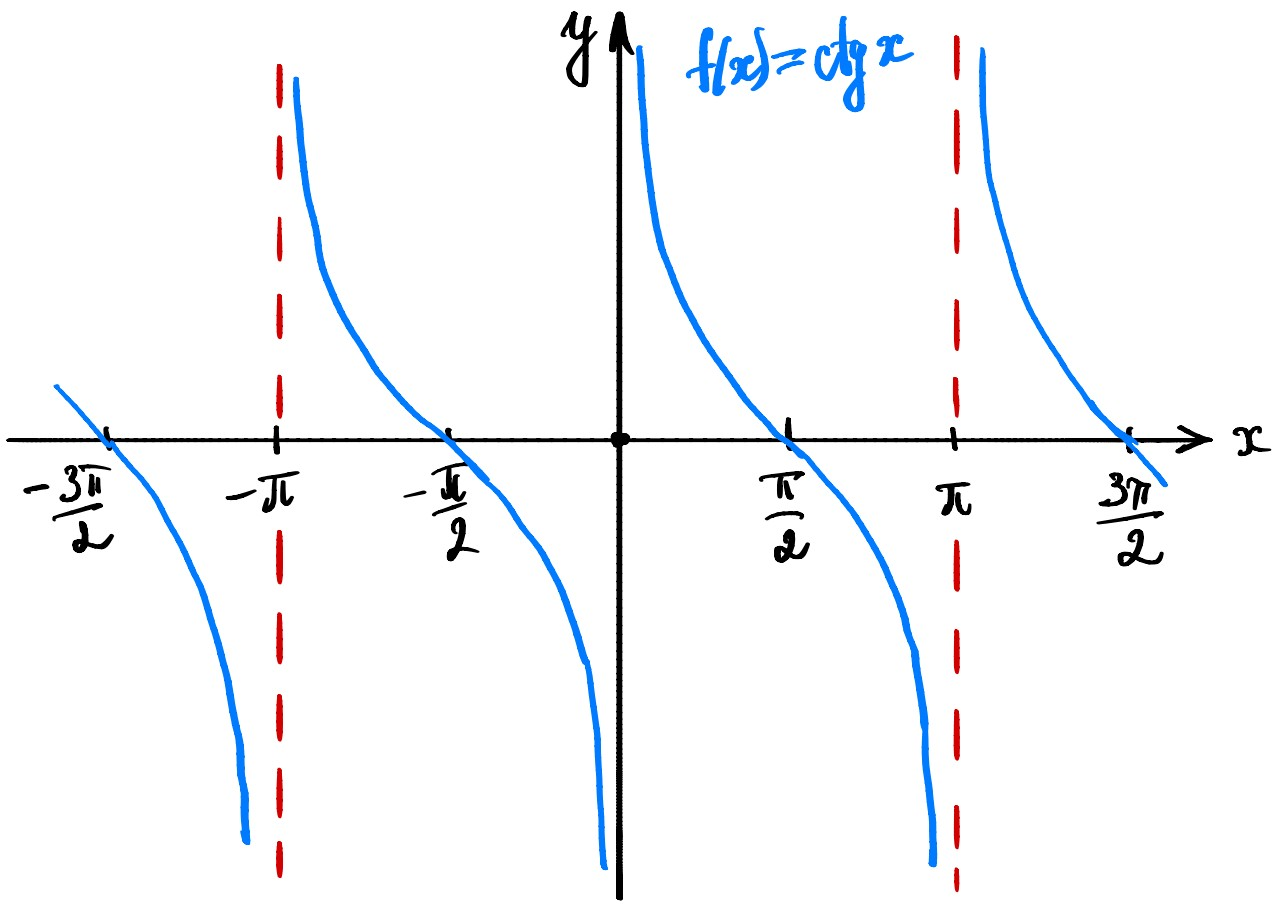
\includegraphics[width=0.6\textwidth]{pictures/pct_cotangence_plot.jpg}
\end{figure}

\subsection*{Обратные тригонометрические функции}\addcontentsline{toc}{subsection}{Обратные тригонометрические функции}

Чтобы получить по значению тригонометрической функции ее аргумент, т.е. угол, нужно знать соответствующую обратную тригонометрическую функцию. Например, мы знаем все стороны в прямоугольном треугольнике, а значит лего можем найти любые соотношения между ними, в том числе значения любых тригонометрических функций углов треугольника. Обратные тригонометрические функции дают возможность узнать и сами углы.

Такие функции называются также как и прямые тригонометрические функции, только с приставкой \textbf{arc} (дуга):
\[\arcsin(x), \quad \arccos(x), \quad \arctg(x), \quad \arcctg(x).\]
\begin{figure}[H]
    \centering
    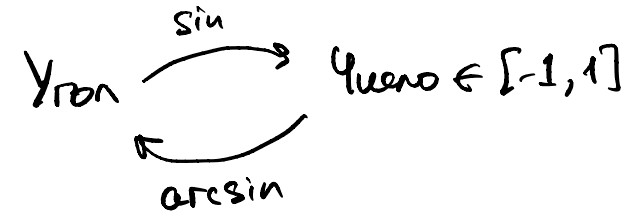
\includegraphics[width=0.4\textwidth]{pictures/pct_inverse_trigonometric.jpg}
\end{figure}

Тут есть, правда, одна проблема. Если снова взглянуть на график, например, синуса, то мы увидим, что каждое его значение повторяется бесконечное число раз. Это понятно, ведь функция периодическая. Отсюда возникает неоднозначность обращения функции. Допустим, мы хотим понять, чему равен $\arcsin(0)$. Тогда мы получаем значения $0, \pm \pi, \pm 2\pi, \ldots$ и что же делать? Здесь, как правило, с неоднозначностью борются очень просто: волевым усилием решается, что берется то значение, которое лежит в промежутке $[-\pi/2, \pi/2]$.

Тогда график арксинуса будет выглядеть таким образом:

TODO: график арксинуса.

График арккосинуса

TODO: график

График арктангенса

TODO: график

График арккотангенса

TODO: график

\subsection*{Зачем это все?}\addcontentsline{toc}{subsection}{Зачем это все?}
Музыка, Фурье, формула Эйлера, механика и т.д.

\setcounter{subpoint}{0}
\subpoint{Движение груза на пружине с дампингом}
Уравнение движения груза на пружине с дампингом:
\[
    mx'' + bx' + kx = 0,
\]
здесь $x(t)$ -- смещение груза, $m$ -- масса груза, $b$ -- дампинг, $k$ -- жесткость пружины (stiffness).

Положим для простоты записи $m = 1$. Тогда уравнение примет вид
\[
x'' + bx' + kx = 0.
\]
Это линейное однородное дифференциальное уравнение второго порядка. Для его решения найдем корни характеристического многочлена
\[
\la^2 + b\la + k = 0.
\]
Это обычное квадратное уравнение, его корни легко находятся через дискриминант:
\[
\la_{1,2} = \frac{-b \pm \sqrt{b^2 - 4k}}{2}.
\]
Тогда, согласно правилу решения уравнений такого рода, все решения описываются так:
\[
x(t) = C_1 e^{-\la_1t} + C_2 e^{-\la_2t},
\]
в случае если $\la_{1,2}$ -- действительные, и
\[
x(t) = e^{-\alpha t}(C_1 \cos(\beta t) + C_2 \sin(\beta t)),
\]
если $\la_{1,2} = \alpha \pm i\beta$ имеют мнимую часть.

Характеристические числа $\la_{1,2}$ будут мнимыми в случае, если
\[
b^2 < 4k,
\]
тогда движение будет осциллирующим. Например, при $k=3$ дампинг не должен превышать значения $2\sqrt 3 \approx 3.5$. А если превысит, то закон движения перестанет носить осциллирующий характер и будет вести себя экспоненциально.

При этом если дампинг равен нулю, т.е. $b = 0$, то движение будет максимально простым:
\[
x(t) = C_1 \cos(\sqrt{k}t) + C_2 \sin(\sqrt{k}t).
\]
и если начальная скорость равна нулю, т.е. $x'(0) = 0$, то находим, что $C_2 = 0$. А если начальное смещение равно $L$, то $C_1 = L$, т.е.
\[
x(t) = L\cos(\sqrt{k}t).
\]
А это просто колебательное движение с амплитудой $L$ и частотой $\frac{\sqrt{k}}{2\pi}$.

\subpoint{Фурье}

\subpoint{Эйлер}

\section*{Криволинейные системы координат}\addcontentsline{toc}{section}{Криволинейные системы координат}
\epigraph{\textit{Решил ты вырваться за предел \\
Осточертевших квадратных форм.}}{— В.А. Лифшиц ''Квадраты''}

Пока что мы продолжаем жить в геометрическом мире, поэтому слово криволинейное можно понимать вполне конкретно --- что-то не прямолинейное. А прямолинейно --- ну ясно же, что такое! Вон, палка прямая валяется.

Система координат, в сущности, это способ закодировать объекты удобным образом. Понятно, что делать это можно по-разному. Как известно, с древности навигация осуществлялась по звездам, города кодировались двумя числами: долготой и широтой. Поэтому сферическая геометрия была развита очень хорошо.

\subsection*{Полярная система координат}\addcontentsline{toc}{subsection}{Полярная система координат}

\subsection*{Сферическая система координат}\addcontentsline{toc}{subsection}{Сферическая система координат}

\subsection*{Цилиндрическая система координат}\addcontentsline{toc}{subsection}{Цилиндрическая система координат}


\section*{Векторы}\addcontentsline{toc}{section}{Векторы}
\subsection*{Развилки в понимании}\addcontentsline{toc}{subsection}{Развилки в понимании}
Вектор это нечто, имеющее величину и направление:
\begin{quote}
\itshape
If anything has magnitude and direction, its magnitude and direction taken together constitute what is called a vector. 

(Gibbs, Elements of Vector Analysis, 1881 \cite{GibbsVectorAnalysis})
\end{quote}

Из этого определения можно попытаться что-то выудить. Раз есть направление, значит, есть какое-то пространство, в котором можно куда-то направляться. Если есть величина, то есть чем измерять. В принципе, это все.

Дальше понятие вектора приобретает различный смысл в зависимости от того, в какой контекст его погрузить. Есть три основные развилки, которые определяют дальнейшую работу с векторами.

Первое это физика. Под векторами понимаются силы, скорость, магнитное поле и т.п. В этой ситуации векторы описывают действия над объектами физического мира.

Второе это геометрия. Здесь вектор это отрезок между двумя точками пространства, имеющий начало и конец. Вектор указывает на то, как из одной точки попасть в другую. Или же можно понимать вектор как перенос одной точки в определенном направлении на определенное расстояние.

И третье --- алгебра. Здесь векторы это нечто, что можно складывать и масштабировать, получая через эти две операции новые векторы. Слова из геометрии типа ''направление'', ''отрезок'' и т.п. здесь уже нелегитимны. Главное --- операции.

\threestars

В каждой из этих трех концепций будут свои развилки, некоторые из которых мы затронем.

Сначала мы вспомним геометрическое представление, операции сложения и растяжения. Поговорим о проекциях и в этом контексте воспользуемся тригонометрией.

Затем перейдем к алгебраическому подходу, где воспользуемся координатным представлением вектора и увидим, как координатные операции связаны с геометрическим представлением. Поговорим о скалярном и векторном произведении, а также о действиях матриц на векторы. Это будет основная часть.

А когда будем говорить про комплесные числа и кватернионы, взглянем на векторы совсем иначе.

\subsection*{Наивное определение и базовые операции}\addcontentsline{toc}{subsection}{Наивное определение и базовые операции}

\subpoint{Определение}

\df Две точки $A$ и $B$, называемые началом и концом, называются вектором $\overrightarrow{AB}$.

\df Длина отрезка $AB$ называется длиной или величиной (magnitude) вектора $\overrightarrow{AB}$ и обозначается $|\overrightarrow{AB}|$.

\df Вектор, у которого начало и конец совпадают, называется нулевым вектором.

\begin{figure}[h] % [h] означает "здесь"
    \centering
    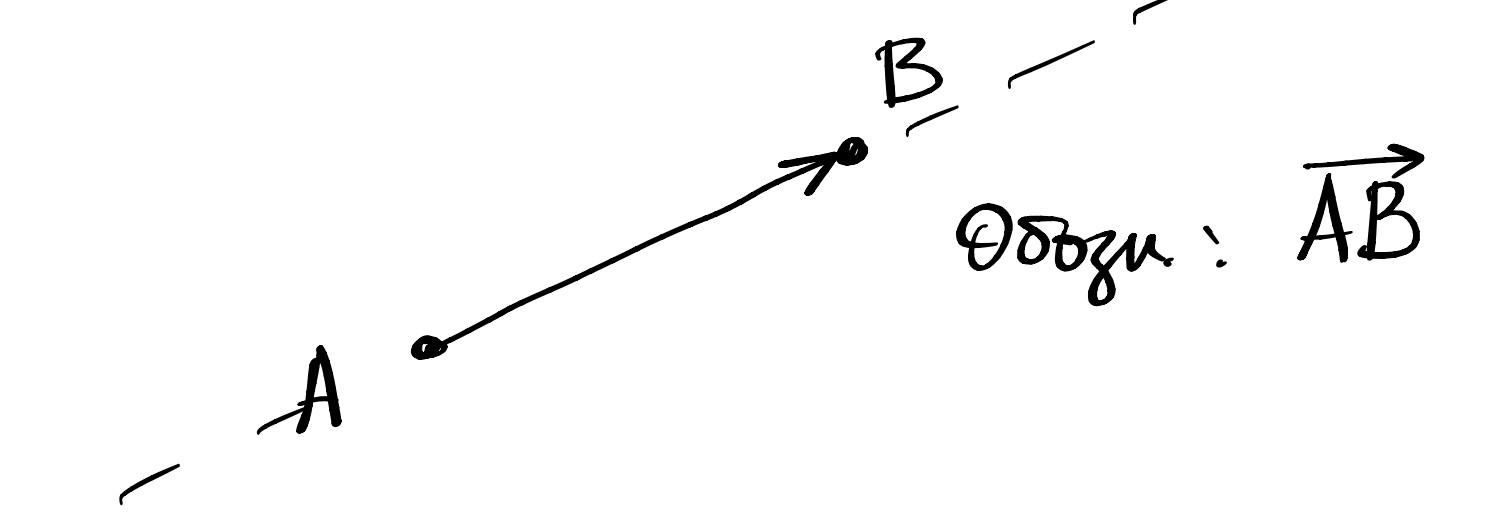
\includegraphics[width=0.6\textwidth]{pictures/vector_df_two_points.jpg}
    \caption{Вектор как две точки}
\end{figure}

\subpoint{Операции}

\df Сложение векторов, имеющих общее начало, осуществляется по правилу параллелограмма. Обозначается
\[
\overrightarrow{AB} + \overrightarrow{AC} = \overrightarrow{AD}.
\]

\begin{figure}[h] % [h] означает "здесь"
    \centering
    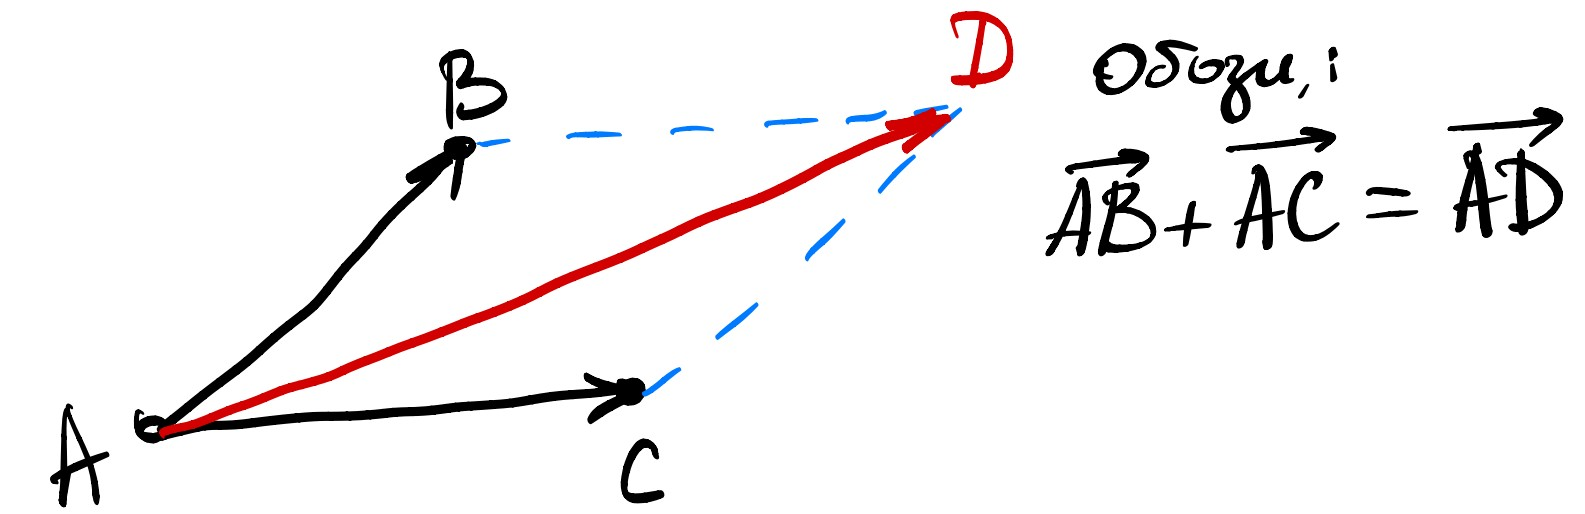
\includegraphics[width=0.6\textwidth]{pictures/pct_vectors_sum.jpg}
    \caption{Правило параллелограмма}
\end{figure}

\df Умножение вектора $\overrightarrow{AB}$ на положительное число $\la$ дает новый вектор с тем же началом и направлением, но длиной $\la |\overrightarrow{AB}|$. Если $\la < 0$, то направление меняется на противопложеное.
\begin{figure}[h] % [h] означает "здесь"
    \centering
    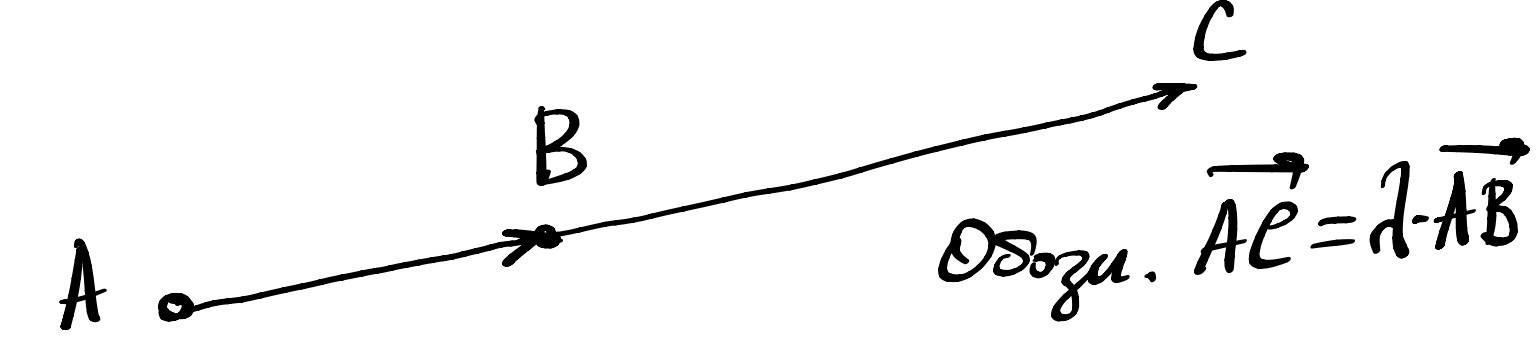
\includegraphics[width=0.6\textwidth]{pictures/pct_vector_scaling.jpg}
    \caption{Умножение вектора на скаляр}
\end{figure}

\subpoint{Как же сложение векторов с разными началами?}

Такое сложение не имеет понятного смысла. Но если воспринимать вектор как направление и величину, то понятно, что один вектор можно задать разными парами точек. Отсюда возникает концепция свободного вектора: все векторы с одинаковым направлением (параллельные) и величиной склеиваются в один.

Свободный вектор можно отложить от любой точки. И вот на таких векторах можно задать сложение:
\begin{figure}[H] % [H] означает "строго здесь"
    \centering
    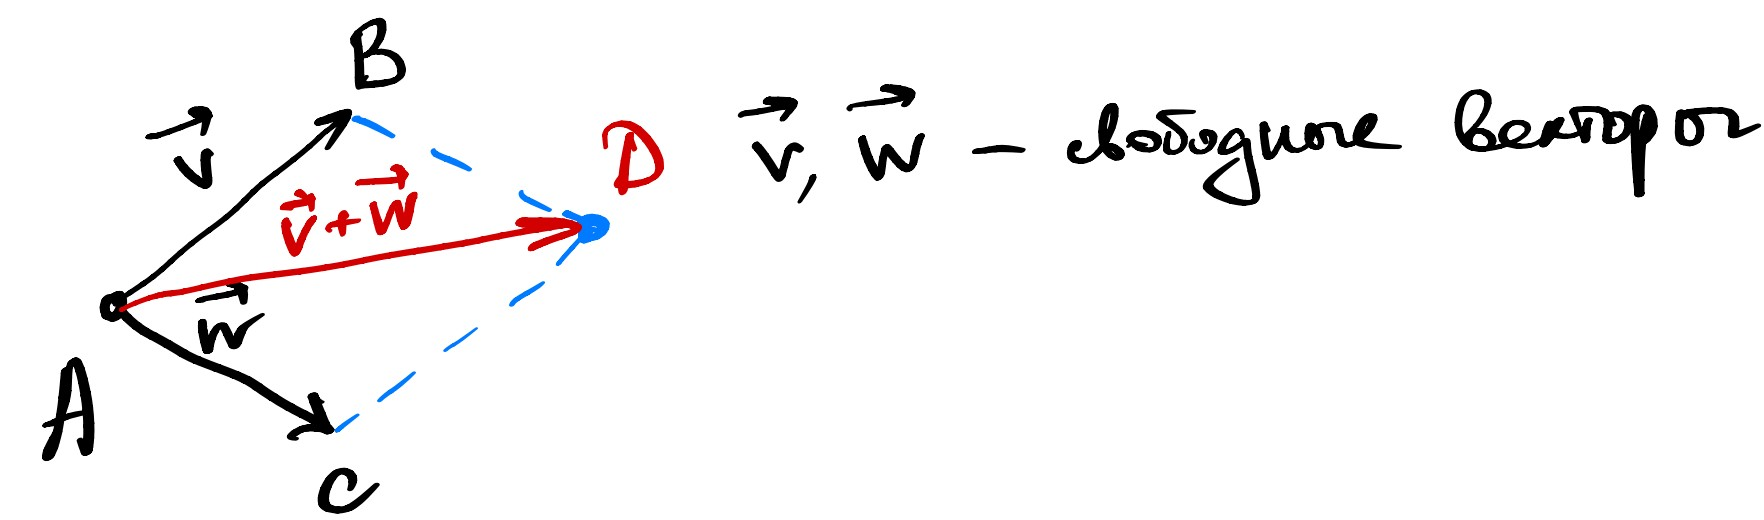
\includegraphics[width=0.6\textwidth]{pictures/pct_free_vectors_sum.jpg}
    \caption{Сложение свободных векторов}
\end{figure}

Можно считать, что все свободные векторы отложены от одной точки:
\begin{figure}[H] % [H] означает "строго здесь"
    \centering
    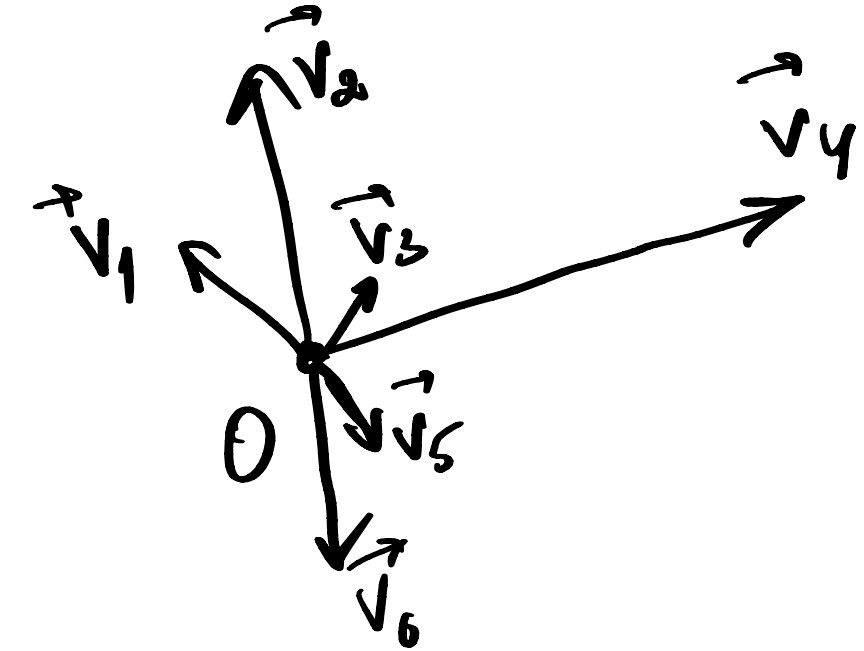
\includegraphics[width=0.3\textwidth]{pictures/pct_multiple_vectors_from_one_point.jpg}
\end{figure}

\subsection*{Вектор и координаты}\addcontentsline{toc}{subsection}{Вектор и координаты}
\setcounter{subpoint}{0}

\subpoint{Что произошло?}

Теперь у точек есть координаты. Для простоты будем считать, что прямоугольные.

Тогда вектор логично определить точно так же, как ранее, но теперь у начала и конца вектора есть координаты $(x,y,z)$.

\subpoint{Свободные векторы}
Мы будем использовать в дальнейшем только свободные векторы, поэтому слово ''свободный'' будем опускать, а как мы отметили, все свободные векторы можно считать отложенными от некоторой конкретной точки. Например, от начала координат, т.е. точки $(0,0,0)$.

Тогда любой вектор, по сути, задается только своим концом. Поэтому вектор можно отождествить с его концом и, соответственно, с его координатами.
\begin{figure}[H] % [H] означает "строго здесь"
    \centering
    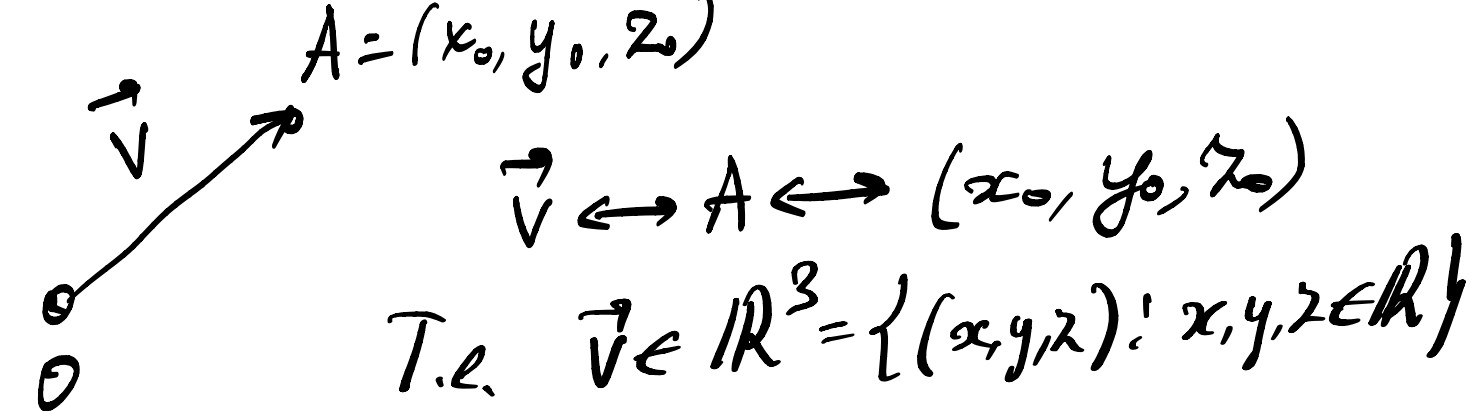
\includegraphics[width=0.6\textwidth]{pictures/pct_coord_vector.jpg}
\end{figure}

\subpoint{Операции}
Сложение двух векторов
\begin{align*}
    &v_1 = (x_1, y_1, z_1)\\
    &v_2 = (x_2, y_2, z_2)
\end{align*}
определяется через покоординатное сложение
\[
w = v_1 + v_2 = (x_1 + x_2, y_1+y_2, z_1+z_2).
\]

Умножение вектора $v = (x,y,z)$ на скаляр $\la \in \R$ дает вектор
\[
w = \la v = (\la x, \la y, \la z).
\]

\subpoint{Векторное пространство и его базис}
\df Множество всех векторов называется векторным пространством (vector space) и обозначается $\R^3$ (читается как ''эр три'').

\df Если через три вектора $e_1, e_2, e_3 \in \R^3$ можно выразить любой вектор $v \in \R^3$, то эти три вектора $\{e_1, e_2, e_3\}$ называются базисом векторного пространства $\R^3$ (basis). 

\ex[Стандартный базис] Зададим базис в $\R^3$:
\begin{align*}
    &e_1 = (1, 0,0)\\
    &e_2 = (0,1,0)\\
    &e_3 = (0,0,1)
\end{align*}
Тогда, если $v = (x,y,z) \in \R^3$, то 
\[
v = xe_1 + ye_2 + ze_3,
\]
а само это представление называется разложением вектора $v$ по базису $e_1, e_2,e_3$.
\begin{figure}[H] % [H] означает "строго здесь"
    \centering
    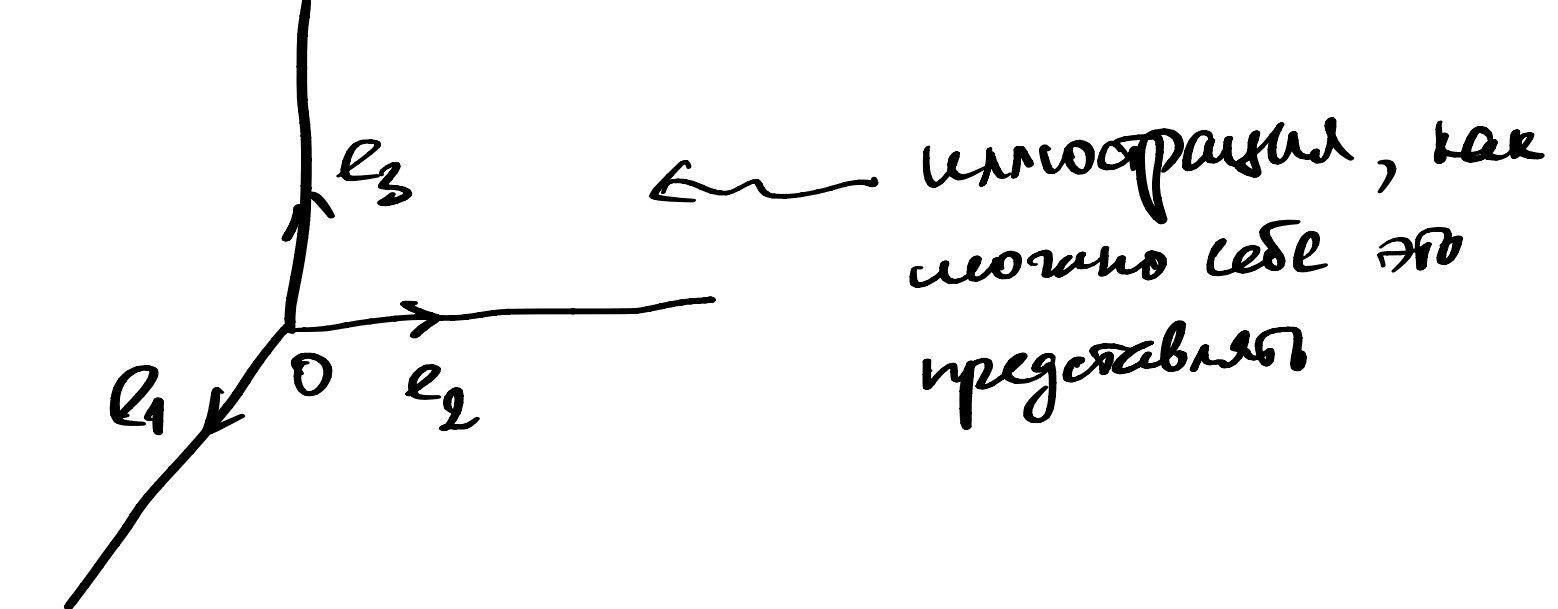
\includegraphics[width=0.6\textwidth]{pictures/pct_vector_orthobasis.jpg}
\end{figure}
Так что, строго говоря, некорректно говорить, что $x,y,z$ -- координаты вектора, ведь координаты есть у точек, а у векторов -- разложение по базису. Разницу между точками и векторами мы обсудим подробнее позже.

\subpoint{Скалярное произведение}
\df Скалярным произведением (scalar product или dot product) двух векторов $v_1 = (x_1,y_1,z_1)$ и $v_2 = (x_2,y_2,z_2)$ называется число, заданное формулой
\[
(v_1,v_2)  \equiv dot(v_1,v_2) := x_1x_2 + y_1 y_2 + z_1 z_2.
\]

Скалярное произведение обладает следующими свойствами
\begin{enumerate}
    \item $(v_1,v_2) = (v_2,v_1)$
    \item $(v_1+v_2, v_3) = (v_1,v_3) + (v_2,v_3)$
    \item $(v,v) = x^2 + y^2 + z^2 \ge 0$
\end{enumerate}

Заметим, что
\begin{align*}
    &(v,e_1) = x \cdot 1 + y \cdot 0 + z \cdot 0 = x\\
    &(v,e_2) = y\\
    &(v,e_3) = z
\end{align*}
То есть скалярное произведение вектора $v$ с базисным вектором $e_i$ дает проекцию $v$ на соответствующее вектору $e_i$ направление. Более подробно мы поговорим о геометрических свойствах скалярного произведения немного дальше.

Об истории термина ''скалярное произведение'' поговорим -- внезапно -- в части о кватернионах.

\subpoint{Длина вектора}
\df Длиной вектора $v = (x,y,z)$ называется число, равное квадратному корню из скалярного квадрата вектора $v$:
\[
|v| = \sqrt{(v,v)} = \sqrt{x^2 + y^2 + z^2}.
\]
Геометрически это определение обосновано теоремой Пифагора.

\noindent\textbf{Вопрос.} Что геометрически представляет из себя множество решений уравнения
\[
|v| = 1?
\]
Указание. Напишите это уравнение в координатном виде (по определению $|v|$).

\subpoint{Формула через косинус}
Из школы известна формула для скалярного произведения в следующем виде
\[
(v_1,v_2) = |v_1| |v_2| \cos \ph,
\]
где $\ph$ -- угол между векторами $v_1$ и $v_2$.

Но как же тогда с определением через координаты? Они совпадают? Ведь совершенно неочевидно равенство
\[
|v_1| |v_2| \cos \ph = x_1x_2 + y_1 y_2 + z_1 z_2.
\]
Доказательство этого факта следует из теоремы косинусов, а именно
\[
|v_2 - v_1|^2 = |v_1|^2 + |v_2|^2 - 2|v_1||v_2| \cos \ph.
\]
\begin{figure}[H] % [H] означает "строго здесь"
    \centering
    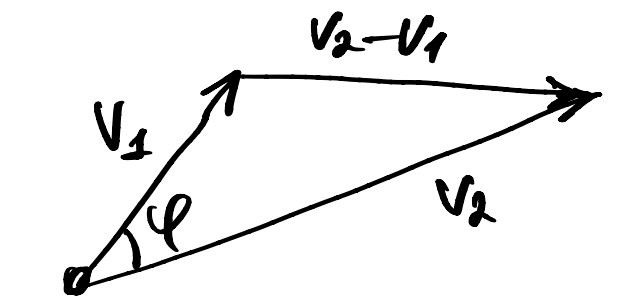
\includegraphics[width=0.3\textwidth]{pictures/pct_cos_theorem.jpg}
\end{figure}

\noindent При этом, с другой стороны,
\[
|v_2-v_1|^2 = (v_2-v_1, v_2-v_1) = |v_2|^2 - 2v_1 v_2 + |v_1|^2.
\]
Приравнивая правые части полученных равенств, получаем
\[
(v_1,v_2) = |v_1| |v_2| \cos \ph.
\]

\NB{Здесь можно наблюдать смешение алгебраических определений и геометрических теорем. Это может у дотошного читателя вызвать тревожный синдром. Действительно, если следовать чисто алгебраическому подходу, мы определили лишь понятие вектора и скалярное произведение на векторах, а понятие угла просто не было неопределено. В этом месте курса линейной алгебры делается ход простой, но малосодержательный для нас: говорится, что косинус угла между двумя векторами есть \textit{по определению}
\[
\cos \ph = \frac{(v_1,v_2)}{|v_1||v_2|}.
\]
А, соответственно, сам угол есть
\[
\ph = \arccos \frac{(v_1,v_2)}{|v_1||v_2|}.
\]}

\noindent\textbf{Вопрос.} Что геометрически означает, что $(v,w) = 0$?

\noindent\textbf{Вопрос.} Как геометрически выглядит множество решений уравнения $(v,x) = 0$?

\noindent\textbf{Упр.} Для вектора $(1,2,3)$ найти какой-нибудь ортогональный. 

\noindent\textbf{Вопрос.} Что говорит об угле между векторами знак скалярного произведения?

\subpoint{Нормализация}
\df Если вектор $v \in \R^3$ имеет длину, равную единице, т.е. $|v| = 1$, то он называется нормированным.

Таким образом, если дан вектор $v$, такой что $|v| = l$, то чтобы его нормировать, нужно умножить его на $1/l$. И тогда вектор
\[
    w = \frac{v}{l}
\]
будет нормированным:
\[
    |w| = \frac{l}{l} = 1.
\]

Говоря на пальцах, смысл нормализации в том, чтобы привести разные объекты к единому стандарту. В случае с векторами, под стандартом понимается длина. Иногда рассматривать векторы с длиной 1 оказывается удобно.

\noindent\textbf{Упр.} Нормализовать вектор $(1,2,3)$. 

\subpoint{Линейная интерполяция}
Рассмотрим два вектора $v,w \in \R^3$. Задача заключается в том, чтобы задать переход от $v$ к $w$ по прямой линии.

Возьмем вектор, который имеет направление от конца $v$ к концу $w$. Этим вектором является вектор $w-v$. Его длина это длина между $v$ и $w$. Поэтому можем задать вектор $u(t)$, зависящий от параметра $t \in [0,1]$ следующим образом:
\[
u(t) = v + t(w-v).
\]

\begin{figure}[H] % [H] означает "строго здесь"
    \centering
    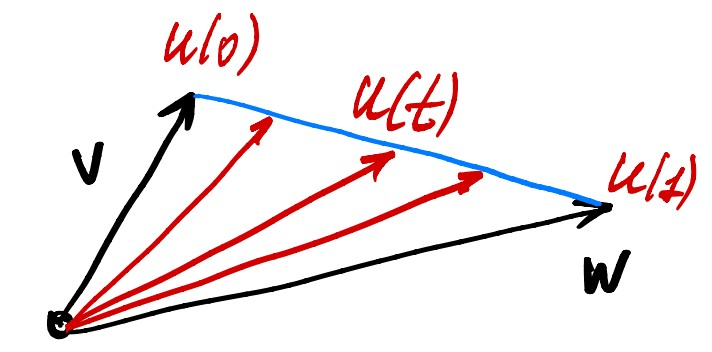
\includegraphics[width=0.4\textwidth]{pictures/pct_linear_interpolation.jpg}
\end{figure}

Здесь с ростом $t$ происходит движение по отрезку между концами $v$ и $w$.

Эта формула может быть переписана иначе:
\[
u(t) = (1-t)v + tw.
\]

\subpoint{Векторное произведение}

Если скалярное произведение векторов есть число, то логично предположить, что можно как-то определить и такое произведение, которое дало бы в результате вектор.

Вообще, под произведением понимается операция, которая обладает некоторыми характерными свойствами. В частности, произведение чисел $a,b \in \R$ обладает свойствами
\begin{itemize}
    \item $ab = ba$ (коммутативность)
    \item $a(bc) = (ab)c$ (ассоциативность)
    \item $a(b+c) = ab + ac$ (дистрибутивность)
\end{itemize}
\noindent\textbf{Упр.} Скалярное произведение обладает всеми тремя этими свойствами.

Но если мы хотим получить в результате вектор, выполнение этих свойств оказывается проблемой. Приходится чем-то жертвовать. Оказывается, что можно определить операцию $\times$, которая почти удовлетворяет всем этим свойствам, за исключением одного момента: операция эта не коммутативна, а антикоммутативна, т.е.
\[
v \times w = -w \times v.
\]

TODO: поискать теорему о том, что нельзя получить коммутативную операцию.

Такая операция называется векторным произведением (vector product или cross product) и обладает следующими важными свойствами:
\begin{itemize}
    \item $v \times w \perp v, w$
    \item $|v \times w| = |v||w|\sin \ph$ -- площадь параллелограмма, построенного на векторах $v,w$ 
\end{itemize}

\begin{figure}[H] % [H] означает "строго здесь"
    \centering
    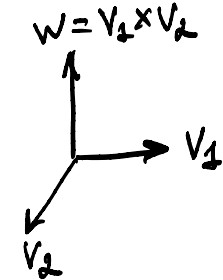
\includegraphics[width=0.15\textwidth]{pictures/pct_cross_product.jpg}
\end{figure}

\noindent\textbf{Вопрос.} Чему равняется $e_1 \times e_2$, $e_1 \times e_3$, $e_2 \times e_3$?

\noindent\textbf{Вопрос.} Чему равняется $e_1 \times e_1$, $e_2 \times e_2$, $e_3 \times e_3$?

\noindent\textbf{Вопрос.} Что геометрически из себя представляет множество решений уравнения $v \times x = 0$?

Мы не дали определения векторного произведения в виде формулы на координаты, однако для ответы на эти вопросы этого не требуется. Далее, в разделе о кватернионах, мы естественным образом получим явную формулу.

\section*{Матрицы}\addcontentsline{toc}{section}{Матрицы}
\subsection*{?}\addcontentsline{toc}{subsection}{?}

\section*{Откуда взялись кватернионы, и вообще?}\addcontentsline{toc}{section}{Откуда взялись кватернионы, и вообще?}



\newpage
\nocite{*}
\printbibliography[nottype=unpublished]

\end{document}